% Consolidated research article. Regenerate with code/assemble_article.py.

% ===== preamble.tex =====
\documentclass[11pt]{article}
\usepackage[T1]{fontenc}
\usepackage{lmodern,microtype}
\usepackage[margin=1in,headheight=15pt]{geometry}
\usepackage{amsmath,amssymb,amsthm,mathtools,mathrsfs}
\usepackage{graphicx,booktabs,longtable,array,enumitem}
\usepackage{xurl}
\usepackage[font=small,labelfont=bf]{caption}
\usepackage[dvipsnames]{xcolor}
\definecolor{Ink}{HTML}{15324C}
\definecolor{Teal}{HTML}{146B72}
\usepackage[colorlinks=true,linkcolor=Ink,citecolor=Teal,urlcolor=Teal,breaklinks=true]{hyperref}
\usepackage[nameinlink,noabbrev]{cleveref}
\usepackage{fancyhdr}
\pagestyle{fancy}\fancyhf{}
\fancyhead[L]{\small Dominant singularities and Euler extrema}
\fancyhead[R]{\small ProveIt continuation}
\fancyfoot[C]{\thepage}
\setlength{\emergencystretch}{2em}
\setlist{itemsep=3pt,topsep=5pt}
\numberwithin{equation}{section}
\newtheorem{theorem}{Theorem}[section]
\newtheorem{lemma}[theorem]{Lemma}
\newtheorem{proposition}[theorem]{Proposition}
\newtheorem{corollary}[theorem]{Corollary}
\newtheorem{conjecture}[theorem]{Conjecture}
\theoremstyle{definition}
\newtheorem{definition}[theorem]{Definition}
\theoremstyle{remark}
\newtheorem{remark}[theorem]{Remark}
\DeclareMathOperator{\Li}{Li}
\DeclareMathOperator{\E}{\mathbb E}
\DeclareMathOperator{\Var}{Var}
\newcommand{\PP}{\mathbb P}
\newcommand{\dd}{\,\mathrm d}
\newcommand{\ii}{\mathrm i}
\newcommand{\src}[1]{\texttt{\detokenize{#1}}}
\newcommand{\stirling}[2]{\genfrac{[}{]}{0pt}{}{#1}{#2}}
\newcommand{\snapshot}{4c173c06cc32c9cea554b39be1837ad2ae897fc1}
\hypersetup{pdftitle={Dominant Singularities, Sharp Euler Extrema, and Lambert Polynomial Zeros},pdfauthor={ProveIt research continuation},pdfsubject={Rigorous continuation, Lerch zero velocities, optimal Euler remainders, Lambert polynomial zeros}}
\begin{document}
\hypersetup{pageanchor=false}
\begin{titlepage}
\vspace*{1cm}
{\large\color{Teal} PROVEIT\quad /\quad RESEARCH CONTINUATION\par}
\vspace{1.0cm}
{\huge\bfseries\color{Ink} Dominant Singularities, Sharp Euler Extrema, and Lambert Polynomial Zeros\par}
\vspace{0.7cm}
{\Large A rigorous continuation of the ProveIt\par
polylogarithm and harmonic-order programs\par}
\vspace{1cm}
{\large Prepared for Vladimir Reshetnikov\par}
\vspace{0.3cm}
{\large October 10, 2026\par}
\vfill
\noindent\textbf{Source baseline.}\quad
\href{https://github.com/VladimirReshetnikov/ProveIt/tree/4c173c06cc32c9cea554b39be1837ad2ae897fc1/Analysis/Polylogarithms/docs/manuscript}{Polylogarithms and their Arithmetic Bridges},
its harmonic-order continuation, and the six archives present in
\src{docs/incoming} at the pinned revision.
\par\medskip
\noindent\textbf{Research status.}\quad
Theorems have ordinary mathematical proofs. Finite algebraic certificates
and high-precision numerical diagnostics have separate roles.
The statements are not presented as Lean formalizations or as claims of
priority over the entire literature.
\par\medskip
\noindent\textbf{Revision.}\quad\texttt{4c173c06cc32c9cea554b39be1837ad2ae897fc1}
\end{titlepage}
\hypersetup{pageanchor=true}
\pagenumbering{roman}


% ===== sections/01_introduction.tex =====
\begin{abstract}
This article continues two analytic programs in the ProveIt polylogarithm
manuscript: sharp Euler remainder estimates at arbitrary real orders,
and the motion of real zeros under harmonic and Lerch deformation.
For the optimal normalized remainder $C_N$, we prove eventual exact
reduction to the outer-order boundary $a=0$, uniqueness of the optimizing
inner order, and the conjectured law
$C_N=1+cN^{-p}+O(N^{-p-\delta})$, with explicit positive constants.
For the pointwise remainder kernel, we prove global convergence of all
maximizers to a unique interior scaled limit, a convergent expansion in
$1/N$, and eventual strict decrease of its optimum. The first later
truncation, $N=2$, has an exact algebraic optimum of degree seven.
For the inverse equation $e^U=A+tU$, an exact rectangular barrier selects
the relevant analytic sheet and its two dominant square-root
singularities for every $A>1$. This makes the repository's conditional
velocity asymptotic unconditional, yields all-order oscillatory
expansions, bounded sign gaps, convergent boundary identities, and an
explicit limiting distribution of the zero-velocity lattice parameters.
The inverse series is identified with earlier work of Kalugin and
Jeffrey, and the coefficient polynomials with Cohen's Lambert
polynomials. For the latter we prove real-rootedness, strict interlacing,
an all-orders fixed-parameter expansion of the largest roots with the
polynomial coefficient degrees conjectured by Cohen, and a Bessel
limit at the smallest-root endpoint. The first two largest-root
corrections are explicit combinations of zeta values. All claims are
separated from numerical evidence and from
questions that remain open. Exact algebraic verification, numerical
diagnostics, source provenance, and integration notes accompany the
article.
\end{abstract}

\tableofcontents
\clearpage
\pagenumbering{arabic}

\section{Research scope, results, and relation to the baseline}
\label{sec:introduction}

The organizing question is how a global extremum or a global inverse
sheet can be recovered from a local asymptotic calculation. In both
problems considered here, the local calculation was substantially
available in the source material, but it did not by itself settle the
global conclusion. For Euler remainders, a trial family on the axis
gave the right candidate correction to the optimal constant; one still
had to exclude all other order parameters. For harmonic zero velocities,
formal critical points and local square-root expansions were known;
one still had to prove that the selected inverse branch actually reaches
exactly the proposed dominant pair. The proofs below supply those
global steps.

\subsection{A fixed and reproducible source comparison}

The repository baseline is revision
\texttt{4c173c06cc32c9cea554b39be1837ad2ae897fc1},
dated October 10, 2026. The review covered the modular manuscript,
its editorial ledger and validation notes, the harmonic-order geometry
continuation, and all six archives then present in \src{docs/incoming}.
The provenance manifest records the paths and Git blob hashes of the
retrieved sources. Statements about what was already proved or left
open refer to this revision, rather than to an evolving branch
\cite{ProveItSnapshot,HarmonicBaseline,UniformBoundsIncoming,SharpEulerIncoming}.

Several substantial problems have already been settled in that baseline.
In particular, the sharp constant uniform in \emph{all} positive real
orders and \emph{all} truncation indices is already known; so are the
$S_2$ and $S_4$ reductions and the certified radial double-extremum
phenomenon. They are not reported here as fresh results. The unresolved
$S_6$ reduction is not claimed. The selected targets are the remaining
global large-index Euler problem and the dominant-sheet question for
diagonal harmonic velocities, together with consequences naturally
forced by their proofs.

\subsection{The main analytic conclusions}

Use the precise normalization of \cref{sec:setup}. The first result is
\[
 C_N=\max_{b>0}R_N(0,b)\quad\hbox{for all sufficiently large }N,
\]
with a unique maximizing order $b_N$. Put
\[
 d=\log(3/2),\qquad p=\frac{\log2}{d},\qquad
 q=\frac{\log3}{\log2},\qquad
 c=\frac{p^p}{(p+1)^{p+1}},\qquad
 \delta=\frac{\log(10/9)}d.
\]
Then
\begin{align}
 b_N&=\frac{\log(Nq)}d+O(N^{-\delta}),\label{eq:intro-b}\\
 C_N&=1+cN^{-p}+O(N^{-p-\delta}).\label{eq:intro-C}
\end{align}
Here $p=1.70951129135\ldots$ and $c=0.167947796543\ldots$.
The positive-quadrant supremum is approached as $a\downarrow0$ and is
not attained there. The proof also gives a necessary scale for any
near-optimal outer order, sharpened to a necessary and sufficient
criterion and a joint profile with exact linear loss $\sqrt\pi$.
It uses probability kernels and positive
Taylor remainders, so no cancellation-sensitive finite Euler sum is
needed as a proof premise.

The pointwise kernel optimum $M_N$ is a different quantity. Its limit is
\[
 M_\infty=1.053861930362711626\ldots>1,
\]
whereas $C_N\to1$. Every global kernel maximizer satisfies
$Nr_N\to3.941064831647250668\ldots$ and
$y_N\to0.145303859259358424\ldots$. The optimized kernel value and
location have convergent expansions in $1/N$ near zero. The exact
degree-seven answer for $M_2$ gives a finite-index anchor for this
asymptotic theory.

For the harmonic problem, let $A=1+h>1$ encode the lattice spacing.
There is a unique $\theta\in(0,\pi)$ such that
\begin{equation}\label{eq:intro-angle}
 \log A=1-\theta\cot\theta+\log\frac\theta{\sin\theta}.
\end{equation}
Writing $a_*=1-\theta\cot\theta$, $u_*=a_*+i\theta$, and
$R=e^{a_*}$, the selected inverse of $e^U=A+tU$ has precisely the
two singularities $Re^{\pm i\theta}$ on its convergence circle.
If $v_n(A)$ is the initial velocity of the $n$th diagonal zero, then
\[
 v_n(A)=\frac{R^{-n}}{\sqrt\pi\,n^{3/2}}
          \Re\!\left(e^{-in\theta}\sqrt{-2u_*}\right)
          +O_A(R^{-n}n^{-5/2}),
\]
with an explicitly selected square root. The article gives its next
coefficient and an algorithm for every subsequent one. The error is
additive; no relative approximation is asserted near a cosine zero.

The same phase describes the distribution of the positive zeros of
the velocity polynomials. In the angle coordinate their limiting
distribution is uniform on $(0,\pi)$. In the logarithmic coordinate
$L=\log A$ its density is
\[
 \frac{\theta}{\pi\bigl((1-\theta\cot\theta)^2+\theta^2\bigr)}.
\]
Thus complex singularity geometry determines both oscillation in the
index and the distribution of real parameters where an initial
velocity vanishes.

The Lambert-polynomial identification also leads to an all-orders
solution of the fixed-parameter extreme-root questions in Cohen's
Conjecture 7.1 \cite{Cohen2021}. If $X_{n,k,j}$ is the $j$th largest
positive root of $L_{n,k}$, then for fixed positive integers $j,k$ and
any fixed $M$,
\begin{equation}\label{eq:intro-Cohen}
 X_{n,k,j}=\frac{n+k-1}{j}+\log n+\gamma-H_{j-1}
       +\sum_{m=1}^{M}\frac{C_{j,m}(k-1)}{n^m}
       +O_{j,k,M}(n^{-M-1}).
\end{equation}
Each $C_{j,m}$ is a polynomial of degree exactly $m-1$. The first
largest-root coefficient is
\[
 C_{1,1}=-\frac32-\zeta(2)-\zeta(3),
\]
and the next coefficient is given explicitly in
\cref{sec:cohen-edges}. Euler's constant occurs only in the leading
shift; every later coefficient lies in a specified algebra generated
by ordinary zeta values. A different endpoint scaling gives
$n^2x_{n,k,j}\to z_{k,j}^2/2$ for the $j$th smallest positive root,
where $z_{k,j}$ is a positive zero of $J_k$. The bulk, large-root,
and Bessel limits have separately stated regimes.

\subsection{Attribution and the meaning of a result here}

Kalugin and Jeffrey's 2012 Lambert-$W$ series already contains the
inverse coefficient array and the convergence-radius criterion after
an explicit change of variables \cite{KaluginJeffrey2012}. Cohen's
Lambert polynomials are the same coefficient polynomials up to a sign
\cite{Cohen2021}. These are substantive identifications, not merely
analogies. They correct a gap in the source comparison and make it
possible to connect the repository's questions to the existing
literature. The barrier proof, its detailed continuation statement,
and the derived velocity and zero-distribution results are presented
with this antecedent made explicit.

Throughout the article, ``proved'' means proved in ordinary mathematics
with the hypotheses stated. The exact polynomial computations have
independent finite verifiers. Numerical calculations illustrate scales,
locate examples, and test formulas; they are not substituted for
global analytic arguments. No assertion of literature-wide priority
or machine-checked formalization is made. The final sections give
precise proposed source amendments and distinguish completed targets
from the remaining finite-index, edge-scaling, and arithmetic questions.


% ===== sections/02_setup.tex =====
\section{A common probability representation for Euler remainders}
\label{sec:setup}

For $a\geq0$ and $b>0$, start in $|z|<1$ with
\begin{equation}\label{eq:polylog-definition}
 F_{a,b}(z)=\sum_{n\geq1}\frac{H_{n-1}^{(b)}}{n^a}z^n,
 \qquad H_m^{(b)}=\sum_{j=1}^m j^{-b},\qquad H_0^{(b)}=0.
\end{equation}
At integer orders this is a depth-two polylogarithmic family; the
probability representation below also handles arbitrary real orders.
Let $T_a,U_b$ be independent gamma variables of rate one and shapes
$a,b$, with $T_0=0$. Put $X=e^{-T_a}$ and $V=e^{-U_b}$. Their moments are
\[
 \E X^{m-1}=m^{-a},\qquad \E V^{m-1}=m^{-b}\qquad(m\geq1).
\]
In particular,
\begin{equation}\label{eq:moment-law}
 \frac{H_{n-1}^{(b)}}{n^a}
    =\E\left[X^{n-1}\frac{1-V^{n-1}}{1-V}\right].
\end{equation}
The quotient at $n=1$ means zero, and otherwise is a finite geometric
sum. Summing in $z$ gives the analytic continuation
\begin{equation}\label{eq:polylog-continuation}
 F_{a,b}(z)=\E\frac{z^2X}{(1-zX)(1-zXV)},
 \qquad z\in\mathbb C\setminus[1,\infty).
\end{equation}
Indeed the integrand is uniformly bounded on compact subsets of the
slit plane, and the identity holds first in the unit disk. Thus the
Gaussian value $g_{a,b}=\Im F_{a,b}(i)$ is unambiguous even when the
corresponding unregularized boundary series fails to converge. Explicitly,
\begin{equation}\label{eq:gaussian-value}
 g_{a,b}=-\E\frac{X^2(1+V)}{(1+X^2)(1+X^2V^2)}.
\end{equation}

For an integer $N\geq1$, define
\begin{align}
 f_n&=\frac{H_{2n}^{(b)}}{(2n+1)^a},\qquad
 d_j=\sum_{n=0}^j(-1)^n\binom jn f_n,
 \label{eq:euler-differences}\\
 E_N&=\sum_{j=0}^{N-1}\frac{d_j}{2^{j+1}},\qquad
 R_N(a,b)=2^N(E_N-g_{a,b}),\qquad
 C_N=\sup_{a,b>0}R_N(a,b).
 \label{eq:euler-normalization}
\end{align}
The sign convention is essential: $E_N$ is an upper approximation to
the negative value $g_{a,b}$. Euler's classical series transformation is
the background for this normalization \cite{DLMFEuler}; here all
identities can be obtained directly from finite sums.

\begin{proposition}[Exact positive remainder and a boundary extension]
\label{prop:gamma-remainder}
With
\[
 W_N(r)=\frac{(1-r)^N}{1+r},\qquad
 K_N(r,v)=\frac{W_N(rv^2)-W_N(r)}{1-v},
\]
one has, for every $a\geq0$, $b>0$, and $N\geq1$,
\begin{equation}\label{eq:gamma-remainder}
 R_N(a,b)=\E K_N(X^2,V)
 =\E\frac{W_N(e^{-2(T_a+U_b)})-W_N(e^{-2T_a})}
             {1-e^{-U_b}}>0.
\end{equation}
Moreover $d_0=0$, $d_j<0$ for $j\geq1$, and $E_N$ decreases to
$g_{a,b}$. The remainder is continuous as $a\downarrow0$ at every
fixed $b>0$.
\end{proposition}
\begin{proof}
The finite binomial identity from \eqref{eq:moment-law} gives
\[
 d_j=\E\frac{(1-X^2)^j-(1-X^2V^2)^j}{1-V}.
\]
Its signs are immediate. Summing the finite geometric series defining
$E_N$ and using \eqref{eq:gaussian-value} proves
\eqref{eq:gamma-remainder}. Decrease of $W_N$ gives strict positivity.
The contraction estimate already established in the manuscript is
\begin{equation}\label{eq:universal-pointwise-bound}
 0\leq K_N(r,v)\leq\frac{1+v}{1+v^2}
       \leq\frac{1+\sqrt2}{2}.
\end{equation}
For a self-contained verification when $N\geq2$, use the power envelope
in \cref{lem:power-envelope} and the positive geometric expansion of
$W_N$ in \cref{lem:kernel-scale}; its $m=2$ envelope is precisely the
first upper bound. For $N=1$, subtraction from that upper bound leaves
\[
 \frac{(1+v)(1-r)(1-rv^2)}
       {(1+v^2)(1+rv^2)(1+r)}\geq0.
\]
Thus $E_N-g_{a,b}=O(2^{-N})$, which proves convergence. Gamma
variables $T_a$ tend in probability to zero as $a\downarrow0$; bounded
convergence using \eqref{eq:universal-pointwise-bound} proves the
boundary continuity.
\end{proof}

The representation and contraction bound are inherited results
\cite{ProveItSnapshot,SharpEulerIncoming}. The following short
conditioning argument supplies a useful direct proof of another
inherited bound, without the signed-measure machinery needed elsewhere
in the manuscript.

\begin{lemma}[The outer-order region $a\geq1$]
\label{lem:outer-order-one}
For all $a\geq1$, $b>0$, and $N\geq1$, one has $R_N(a,b)<1$.
\end{lemma}
\begin{proof}
Decompose $T_a=T_1+T_{a-1}$ independently. Since $e^{-T_1}$ is
uniform on $(0,1)$, condition on $Z=e^{-T_{a-1}}\in(0,1]$ and
$V=v\in(0,1)$. The conditional expectation of the kernel is
\begin{align*}
 &\int_0^1 K_N(Z^2u^2,v)\,du\\
 &\qquad=\frac{v^{-1}\int_0^{Zv}W_N(t^2)\,dt
                         -\int_0^Z W_N(t^2)\,dt}{Z(1-v)}\\
 &\qquad\leq\frac1{Zv}\int_0^{Zv}W_N(t^2)\,dt<1.
\end{align*}
The first inequality uses $W_N\geq0$, and the second uses
$W_N(t^2)<1$ for $t>0$. Taking expectations proves the claim.
\end{proof}

\subsection{Three constants that must be distinguished}

Write
\[
 C_N^{\mathrm{ax}}=\max_{b>0}R_N(0,b),\qquad
 M_N=\max_{(r,v)\in[0,1]^2}K_N(r,v),
\]
where existence of the axis maximum is proved below. The boundary
continuity and the probability representation give
\begin{equation}\label{eq:constant-hierarchy}
 C_N^{\mathrm{ax}}\leq C_N\leq M_N.
\end{equation}
The already known all-index constant is
$C_*:=\sup_{N\geq1}C_N=1.13656\ldots$, attained only after adjoining
$a=0$ and then at $N=1$ and a unique inner order
\cite{ProveItSnapshot,SharpEulerIncoming}. The present global theorem
proves $C_N^{\mathrm{ax}}=C_N$ for sufficiently large $N$ and $C_N\to1$. The separate
kernel theorem proves $M_N\to M_\infty>1$. Maximization before and after
gamma averaging cannot be interchanged without proof.


% ===== sections/03_global_euler.tex =====
\section{Global optimization of the real-order Euler remainder}
\label{eul:sec:global}
The matching upper asymptotic was explicitly left open as Conjecture
\texttt{conj:euler-rate} in the incoming uniform-bounds report
\cite{UniformBoundsIncoming}. Its axis lower bound already identified
the candidate exponent and leading amplitude. The additional ingredients
here are global localization over both orders, a positive loss that
forces the outer order to the boundary, and uniform derivative control
for the inner-order optimization. The region $a\geq1$ is excluded by
\cref{lem:outer-order-one}, whose direct proof was given above.

\subsection{Statement}
Put
\[
 d=\log(3/2),\qquad p=\frac{\log2}{d},\qquad
 q=\frac{\log3}{\log2},\qquad
 c=(1-q^{-1})q^{-p},\qquad
 \delta=\frac{\log(10/9)}d>0,
\]
and
\[
 \widehat b_N=\frac{\log(Nq)}d.
\]
Thus $p=1.7095112913514547\ldots$,
$c=0.1679477965425128\ldots$, and
$\delta=0.2598510045646633\ldots$.
For independent gamma variables of rate one, with shape zero interpreted
as the point mass at zero, define
\[
 W_N(z)=\frac{(1-z)^N}{1+z},\qquad
 F_N(t)=W_N(e^{-2t}),\qquad
 J_N(a)=\E F_N(T_a).
\]
The existing all-order Euler formula is
\begin{equation}\label{eul:eq:R}
 R_N(a,b)=\E\frac{F_N(T_a+U_b)-F_N(T_a)}{1-e^{-U_b}},
 \qquad a\geq0,\quad b>0.
\end{equation}
In particular $J_N(0)=F_N(0)=0$.

\begin{theorem}[Eventual exact axis reduction]\label{eul:thm:main}
There is an integer $N_0$ such that for every $N\geq N_0$,
\begin{equation}\label{eul:eq:axisexact}
 C_N:=\sup_{a,b>0}R_N(a,b)
   =\max_{b>0}R_N(0,b).
\end{equation}
The maximum on the right is attained at exactly one $b_N$, and
\begin{align}
 b_N&=\widehat b_N+O(N^{-\delta}),\label{eul:eq:bn}\\
 C_N&=1+cN^{-p}+O(N^{-p-\delta}).\label{eul:eq:cn}
\end{align}
For $N\geq N_0$ the supremum on the positive quadrant is not attained;
on the domain $a\geq0,b>0$ its unique maximizer is $(0,b_N)$.
Moreover $C_{N+1}<C_N$ for every sufficiently large $N$.
\end{theorem}

\begin{theorem}[Scale of near maximizers]\label{eul:thm:near}
If $a_N,b_N'>0$ and
\[
 C_N-R_N(a_N,b_N')=o(N^{-p}),
\]
then
\[
 b_N'-\widehat b_N\longrightarrow0,
 \qquad
 a_N=o\!\left(N^{-(p-1/2)}\log N\right).
\]
The same assertion holds with $a_N=0$ allowed.  This accuracy requirement
is essential: the incoming moving-order phase law already gives many
sequences with $R_N\to1$ and $a_N$ increasing to infinity.
\end{theorem}

\subsection{Elementary bounds and a gamma expansion}
The function $F_N$ increases from zero to one.  Direct differentiation
gives $0\leq F_N'\leq4$, uniformly in $N$, and $F_N'$ tends uniformly
to zero on every fixed bounded interval.  These facts also follow from
\[
 F_N'(t)=\frac{2z(1-z)^{N-1}\{N+1+(N-1)z\}}{(1+z)^2},
 \qquad z=e^{-2t}.
\]
For $N\geq2$ use $Nz(1-z)^{N-1}\leq1$; for $N=1$ the bound is
immediate.

For $b>1$ expand $(1-e^{-U_b})^{-1}$ positively.  Exponential tilting
changes $U_b$ to a gamma variable $U_b^{(m)}$ of rate $m$, with total
weight $m^{-b}$.  Consequently
\begin{equation}\label{eul:eq:seriesR}
 R_N(a,b)=\sum_{m\geq1}m^{-b}
  \{\E F_N(T_a+U_b^{(m)})-J_N(a)\}.
\end{equation}
Every term in braces lies in $[0,1]$, and the term $m=1$ is
$J_N(a+b)-J_N(a)$.  Therefore
\begin{equation}\label{eul:eq:rough}
 R_N(a,b)\leq\zeta(b),\qquad
 R_N(a,b)\leq J_N(a+b)-J_N(a)+\zeta(b)-1.
\end{equation}
For $b\geq2$ the elementary integral estimate gives
\begin{equation}\label{eul:eq:zetabound}
 \zeta(b)-1\leq2^{-b}\left(1+\frac2{b-1}\right)\leq3\,2^{-b}.
\end{equation}
We will use the sharper factor $2$ once $b\to\infty$.

The function $W_N$ is convex and
\begin{equation}\label{eul:eq:etaylor}
 W_N(z)=1-(N+1)z+e_N(z),\qquad
 0\leq e_N(z)\leq B_Nz^2,
 \quad B_N=\frac{N^2+N+2}{2}.
\end{equation}
Furthermore $e_N$ is nondecreasing on $[0,1]$.
For completeness, $W_N'(0)=-(N+1)$ and
$0\leq W_N''(z)\leq W_N''(0)=N^2+N+2$.
For $N\geq2$ the latter follows by differentiating
$(1-z)^N/(1+z)$ twice and bounding each positive term at zero;
for $N=1$ use $H_1(z)=2/(1+z)-1$.
Convexity gives $W_N'(z)\geq W_N'(0)$, proving $e_N'\geq0$.

Write $S_j(b)=\sum_{m\geq j+1}m^{-b}$.  Substitution of
\eqref{eul:eq:etaylor} in \eqref{eul:eq:R}, with $x=e^{-T_a}$ and
$v=e^{-U_b}$, gives the exact identity
\begin{equation}\label{eul:eq:exactexpansion}
 R_N(a,b)=\zeta(b)(1-J_N(a))
 -(N+1)3^{-a}S_2(b)+\eta_N(a,b),
\end{equation}
where
\begin{equation}\label{eul:eq:eta}
 \eta_N(a,b)=\E\frac{e_N(x^2v^2)}{1-v},\qquad
 0\leq\eta_N(a,b)\leq B_N5^{-a}S_4(b).
\end{equation}
This is valid for $b>1$.  Gamma addition couples $T_{a_2}\geq T_{a_1}$
when $a_2>a_1$.  Since $e_N$ is nondecreasing, it also proves the
important exact monotonicity
\begin{equation}\label{eul:eq:etamonotone}
 a\longmapsto\eta_N(a,b)\quad\hbox{is nonincreasing}.
\end{equation}

\subsection{Uniform localization of every competitive pair}
Call a pair competitive if
\begin{equation}\label{eul:eq:competitive}
 R_N(a,b)\geq1+\frac c2N^{-p}.
\end{equation}
The axis lower asymptotic already proved in the incoming report implies
that competitive pairs exist for all sufficiently large $N$, including
positive $a$ by continuity at $a=0$.
By \cref{lem:outer-order-one}, every competitive pair has $0\leq a<1$.
Set $\ell=\log N$ and $L=\ell/2$.

\begin{lemma}[A fixed logarithmic band]\label{eul:lem:band}
There are fixed constants $M_-,M_+>0$ such that for all sufficiently
large $N$, every competitive pair satisfies
\[
 0\leq a<1,\qquad
 \widehat b_N-M_-\leq b\leq\widehat b_N+M_+.
\]
One may take $M_-=10$ and $M_+=5$ after increasing the unspecified
threshold in $N$.
\end{lemma}
\begin{proof}
We first prove that $R_N(a,b)<1$ whenever $0\leq a\leq1$ and
$b\leq\widehat b_N-10$, for all sufficiently large $N$.

\paragraph{Bounded inner orders, $0<b\leq2$.}
Gamma addition permits a coupling with $T_a\leq T_1$ and
$U_b\leq U_2$, independently.  The mean-value formula and
$u/(1-e^{-u})\leq1+u$ imply
\[
 \frac{F_N(T_a+U_b)-F_N(T_a)}{1-e^{-U_b}}
 \leq(1+U_2)\sup_{0\leq t\leq T_1+U_2}F_N'(t).
\]
The right side is independent of the smaller shapes, bounded by the
integrable variable $4(1+U_2)$, and tends to zero almost surely.
Dominated convergence proves uniform convergence $R_N\to0$ on this
rectangle.

\paragraph{Small growing orders, $2\leq b\leq\ell/4$.}
The second inequality of \eqref{eul:eq:rough}, stochastic monotonicity of
$J_N$, and $\zeta(2)-1\leq3/4$ give
\[
 R_N(a,b)\leq J_N(1+\ell/4)+3/4.
\]
The first term tends to zero.  Indeed a gamma variable of shape
$1+\ell/4$ divided by $\ell$ tends to $1/4$ in probability, by its
mean and variance; on $t\leq3\ell/8$,
$F_N(t)\leq\exp(-N^{1/4})$, and the probability of the complement
tends to zero.  Hence this whole range eventually has $R_N<1$.

\paragraph{Intermediate growing orders, $\ell/4\leq b\leq2\ell$.}
Put $s=a+b=\alpha\ell$.  For large $N$,
$1/4\leq\alpha\leq2+1/\ell$.  For $t\in[L,L+1]$,
\[
 1-F_N(t)\geq d_0:=1-\exp(-e^{-2})>0.
\]
Since $s\geq1$, the gamma density on that interval gives
\begin{equation}\label{eul:eq:tailwindow}
 1-J_N(s)\geq
 d_0e^{-1}N^{-1/2}\frac{L^{s-1}}{\Gamma(s)}.
\end{equation}
The real Stirling bound $\Gamma(s)\leq A s^{s-1/2}e^{-s}$ for
$s\geq1$, with any fixed valid constant $A$, yields uniformly
\[
 1-J_N(s)\geq A_1\ell^{-1/2}\exp\{-\ell I(\alpha)\},
 \qquad I(\alpha)=\tfrac12-\alpha+\alpha\log(2\alpha).
\]
Comparison with $2^{-b}=2^a\exp(-\alpha\ell\log2)$ shows
\[
 \frac{1-J_N(a+b)}{2^{-b}}
 \geq A_2\ell^{-1/2}\exp\{\ell Q(\alpha)\},
 \qquad Q(\alpha)=\alpha-\tfrac12-\alpha\log\alpha.
\]
This tends uniformly to infinity.  To check uniformity explicitly,
$Q$ is concave and positive at both endpoints of $[1/4,2]$:
\[
 Q(1/4)=(\log4-1)/4>0,\qquad Q(2)=3/2-2\log2>0.
\]
By continuity and concavity, its minimum on
$[1/4,2+1/\ell]$ is bounded below by a fixed positive number for all
large $\ell$.  For example $Q\geq1/40$ on $[1/4,21/10]$;
the last upper endpoint contains the required interval when $\ell\geq10$.
Thus \eqref{eul:eq:zetabound} gives
$1-J_N(a+b)>\zeta(b)-1$ uniformly in this range.  Equation
\eqref{eul:eq:rough} now proves $R_N(a,b)<1$.

\paragraph{Upper logarithmic range, $2\ell\leq b\leq\widehat b_N-10$.}
Average \eqref{eul:eq:etaylor} with a gamma shape $s=a+b$ to obtain
\[
 1-J_N(s)\geq(N+1)3^{-s}-B_N5^{-s}.
\]
For $s\geq2\ell$, the ratio of the second term to the first is at most
\[
 \frac{B_N}{N+1}(3/5)^{2\ell}
   =O\!\left(N^{1-2\log(5/3)}\right)=o(1),
\]
since $2\log(5/3)>1$.  With $0\leq a\leq1$ this gives, for large $N$,
\[
 1-J_N(a+b)\geq\frac N4\,3^{-b}.
\]
On the other hand $\zeta(b)-1\leq2\,2^{-b}$ here.  At
$b\leq\widehat b_N-10$,
\[
 \frac{(N/4)3^{-b}}{2^{-b}}
 \geq\frac{(3/2)^{10}}{4q}>2.
\]
Thus the gamma loss again exceeds $\zeta(b)-1$, and
\eqref{eul:eq:rough} proves $R_N<1$.

These four ranges cover every $b\leq\widehat b_N-10$ for all large
$N$, because $1/d>2$.  They prove the lower edge of the band.
For a competitive pair, the first inequality of \eqref{eul:eq:rough} and
$\zeta(b)-1\leq2\,2^{-b}$ imply
\[
 \frac c2N^{-p}\leq2\,2^{-b}.
\]
Using $2^{-\widehat b_N}=q^{-p}N^{-p}$, this gives
\[
 b-\widehat b_N\leq\log_2\frac4{1-q^{-1}}<5.
\]
This proves the upper edge and completes the proof.
\end{proof}

\subsection{A positive loss that forces the boundary maximum}
\begin{lemma}[Uniform lower bound for the outer-order loss]\label{eul:lem:slope}
There is a fixed $D>0$ such that, for all sufficiently large $N$,
\[
 J_N(a)\geq D a\frac{N^{-1/2}}{\log N}
 \qquad(0\leq a\leq1).
\]
\end{lemma}
\begin{proof}
The assertion is immediate at $a=0$.  For $0<a\leq1$, integrate the
positive gamma representation over $t\in[L+1,L+2]$.
On this interval, Bernoulli's inequality gives
\[
 F_N(t)\geq F_N(L+1)\geq h_0:=\frac{1-e^{-2}}2>0.
\]
Log-convexity of $\Gamma$ and $\Gamma(1)=\Gamma(2)=1$ imply
$\Gamma(a+1)\leq1$, so $1/\Gamma(a)=a/\Gamma(a+1)\geq a$.
For large $N$, also $t^{a-1}\geq1/t\geq1/(L+2)$ on the interval,
and $e^{-t}\geq e^{-2}N^{-1/2}$.  Therefore
\[
 J_N(a)\geq h_0e^{-2}\frac{aN^{-1/2}}{L+2},
\]
which proves the claimed uniform bound.
\end{proof}

\begin{proposition}[Strict comparison with the axis]\label{eul:prop:decrease}
For all sufficiently large $N$ and every
$b\in[\widehat b_N-10,\widehat b_N+5]$,
\begin{equation}\label{eul:eq:gap-a}
 R_N(0,b)-R_N(a,b)
 \geq d_{\mathrm{loss}} a\frac{N^{-1/2}}{\log N}
 \quad(0\leq a\leq1),
\end{equation}
for a fixed constant $d_{\mathrm{loss}}>0$.
\end{proposition}
\begin{proof}
Subtract \eqref{eul:eq:exactexpansion} at $a$ and at zero, and use
\eqref{eul:eq:etamonotone}, Lemma~\ref{eul:lem:slope}, $\zeta(b)\geq1$, and
$1-3^{-a}\leq a\log3$.  This gives
\[
 R_N(a,b)-R_N(0,b)
 \leq a\left\{
 -D\frac{N^{-1/2}}{\log N}+(N+1)(\log3)S_2(b)\right\}.
\]
Uniformly in the stated band,
$S_2(b)=O(3^{-b})$ and $N3^{-b}=O(N^{-p})$.
Since $p>1/2$, the positive term is smaller than half the negative
one for all sufficiently large $N$.  Take $d_{\mathrm{loss}}=D/2$.
\end{proof}

\subsection{Axis optimization with controlled derivatives}
On the axis, the exact kernel is
\[
 R_N(0,b)=\E k_N(e^{-U_b}),\qquad
 k_N(v)=\frac{(1+v)(1-v^2)^{N-1}}{1+v^2}.
\]
For every fixed $N\geq2$ this is continuous in $b>0$, tends to zero
as $b\downarrow0$, and tends to one as $b\to\infty$.
The last limit follows from bounded convergence under gamma addition,
or directly from the moment expansion below.  That expansion also
shows $R_N(0,b)>1$ for sufficiently large $b$, with $N$ fixed.
Thus its global maximum is attained at a finite positive $b$.

\begin{proposition}[Unique nondegenerate axis maximum at every index]
\label{eul:prop:axisunique}
For every integer $N\geq1$, $b\mapsto R_N(0,b)$ has exactly one
stationary point.  It is a nondegenerate global maximum, of height
strictly greater than one.
\end{proposition}
\begin{proof}
For $N\geq2$, the sign of $k_N'(v)$ is that of
\[
 h_N(v)=1-(2N+1)v+v^2+(3-2N)v^3.
\]
Its derivative is strictly negative on $[0,1]$, while
$h_N(0)=1$ and $h_N(1)=4-4N<0$.
Thus $\widetilde k_N(t)=k_N(e^{-t})$ increases from zero to a unique maximum
greater than one, then decreases to one.  For $N=1$ the same shape
statement holds with value one at both endpoints; use
$k_1'(v)=(1-2v-v^2)/(1+v^2)^2$.

Fix $b$ and write $M=\E \widetilde k_N(U_b)=R_N(0,b)$.
Differentiation under the gamma integral gives
\[
 R_N'(0,b)=\E\{(\widetilde k_N(U_b)-M)\log U_b\},
\]
where the notation here means the derivative in $b$ of the axis
function.  If $M\leq1$, then $\widetilde k_N(t)-M$ has exactly one finite sign
change, from negative to positive, at a point $t_0$.
Subtracting $\log t_0$ in this expectation makes its integrand
strictly positive except at the crossing, so the derivative is
positive.  For $N=1$, $M>1$ automatically.

At any stationary point we therefore have $M>1$.  The function
$\widetilde k_N(t)-M$ then has exactly two crossings $t_1<t_2$, with signs
negative, positive, negative.  Both its gamma average and its
logarithmic first moment vanish at the stationary point.  A second
differentiation consequently gives
\begin{align*}
 \frac{d^2}{db^2}R_N(0,b)
 &=\E\{(\widetilde k_N(U_b)-M)(\log U_b)^2\}\\
 &=\E\{(\widetilde k_N(U_b)-M)(\log U_b-\log t_1)
                          (\log U_b-\log t_2)\}<0.
\end{align*}
The last integrand is strictly negative away from the crossings.
All differentiations are justified by boundedness of $\widetilde k_N$ and the
finite logarithmic moments of gamma laws locally in $b>0$.

The endpoint limits and a value above one guarantee at least one
interior maximum.  Every stationary point has negative second
derivative, so there cannot be two: between two strict maxima there
would be a stationary minimum (or the derivative would have to
cross from negative to positive).  This proves the assertion.
\end{proof}

The incoming Taylor identity, restated to track its derivatives, is
\begin{equation}\label{eul:eq:axisexp}
 R_N(0,b)=1+2^{-b}-N3^{-b}-N4^{-b}+\varepsilon_N(b),
\end{equation}
where
\begin{equation}\label{eul:eq:axisrem}
 0\leq\varepsilon_N(b)\leq
 A_N(5^{-b}+6^{-b}),\qquad A_N=(N^2-N+2)/2.
\end{equation}
Indeed, for $G_N(z)=(1-z)^{N-1}/(1+z)$,
$G_N(z)=1-Nz+r_N(z)$ with
$0\leq r_N(z)\leq A_Nz^2$; multiply by $1+v$, set $z=v^2$, and
integrate the gamma moments.

For $k=0,1,2$, the remainder has the derivative bound
\begin{equation}\label{eul:eq:derivative-bound}
 |\varepsilon_N^{(k)}(b)|\leq A_k N^2\,5^{-b}
 \qquad(b\geq1),
\end{equation}
with constants $A_k$ independent of $N,b$.
To see this without differentiating an inequality, write the exact
nonnegative remainder as
\[
 \varepsilon_N(b)=\frac1{\Gamma(b)}\int_0^\infty
 t^{b-1}e^{-t}w_N(t)\dd t,
 \quad 0\leq w_N(t)\leq A_N(e^{-4t}+e^{-5t}).
\]
The first two derivatives of the gamma density multiply it by
\[
 \log t-\psi(b),\qquad
 (\log t-\psi(b))^2-\psi_1(b).
\]
After exponential tilting to rate $m\in\{5,6\}$, the score has
mean $-\log m$ and variance $\psi_1(b)\leq\psi_1(1)=\pi^2/6$.
Cauchy--Schwarz therefore bounds the absolute first score moment by
$\log m+\pi/\sqrt6$, and the absolute second derivative factor by
$(\log m)^2+\pi^2/3$.  These bounds prove
\eqref{eul:eq:derivative-bound}.  Differentiation is justified by the same
locally integrable domination.

For bounded real $s$, equations \eqref{eul:eq:axisexp}--\eqref{eul:eq:derivative-bound}
give, uniformly with two derivatives in $s$,
\begin{equation}\label{eul:eq:C2profile}
 N^p\{R_N(0,\widehat b_N+s)-1\}
   =f(s)+O(N^{-\delta}),
\end{equation}
where
\[
 f(s)=q^{-p}2^{-s}-q^{-(p+1)}3^{-s}.
\]
For the error exponents, $N4^{-\widehat b_N}=O(N^{-p-(p-1)})$
and $N^25^{-\widehat b_N}=O(N^{-p-\delta})$,
with $p-1>\delta>0$.  The same statements hold after up to two
derivatives.

The function $f$ has its unique global maximum at $s=0$:
\[
 f(0)=c,\qquad f'(0)=0,\qquad
 f''(0)=-(\log2)\,d\,q^{-p}<0.
\]
Its derivative has exactly one zero because its two exponential terms
have distinct rates.

\subsection{Completion of the proofs}
\begin{proof}[Proof of Theorem~\ref{eul:thm:main}]
The axis value at $\widehat b_N$ is
$1+cN^{-p}+O(N^{-p-\delta})$, so its maximum exceeds
$1+(c/2)N^{-p}$ for all sufficiently large $N$.
Every pair that could exceed this axis maximum is therefore competitive.
Lemma~\ref{eul:lem:band} places it in $0\leq a<1$ and the fixed
logarithmic band.  Proposition~\ref{eul:prop:decrease} gives
$R_N(a,b)\leq R_N(0,b)$ there, strictly for $a>0$.
Pairs outside that competitive class cannot be maximizers.  This proves
the exact global reduction \eqref{eul:eq:axisexact}; continuity at $a=0$
shows that the same value is the supremum over $a,b>0$.

Every axis maximizer also lies in the band of Lemma~\ref{eul:lem:band}.
Uniform convergence in \eqref{eul:eq:C2profile}, compactness of the band,
and the unique maximum of $f$ force every maximizing offset
$b-\widehat b_N$ to tend to zero.  In a fixed small neighborhood of
zero, $f''$ is bounded above by a strictly negative constant.  The
uniform second derivative version of \eqref{eul:eq:C2profile} makes the
axis function strictly concave there for all large $N$.
Since all of its global maxima lie there, its global maximum is unique.
Denote it by $b_N$.
Its first derivative vanishes, so
$f'(b_N-\widehat b_N)=O(N^{-\delta})$.
The nonzero value of $f''(0)$ and the mean-value theorem imply
\eqref{eul:eq:bn}.  Equation \eqref{eul:eq:C2profile} then gives
\eqref{eul:eq:cn}.

The strict axis comparison proves nonattainment in the positive quadrant
and uniqueness on the closed axis domain.  Finally, for each finite
$b>0$, $k_{N+1}(v)=(1-v^2)k_N(v)<k_N(v)$ on $(0,1)$.
At the finite maximizer of the $(N+1)$st axis problem,
\[
 C_{N+1}=R_{N+1}(0,b_{N+1})
  <R_N(0,b_{N+1})\leq C_N.
\]
This applies whenever both adjacent indices have the axis reduction.
\end{proof}

\begin{proof}[Proof of Theorem~\ref{eul:thm:near}]
The assumed accuracy makes the pair competitive for all large $N$.
It therefore lies in the fixed band and $0\leq a_N<1$.
By \eqref{eul:eq:gap-a},
\[
 C_N-R_N(a_N,b_N')
 \geq R_N(0,b_N')-R_N(a_N,b_N')
 \geq d_{\mathrm{loss}}a_N\frac{N^{-1/2}}{\log N}.
\]
This yields the stated little-oh estimate on $a_N$.
Moreover
$0\leq C_N-R_N(0,b_N')\leq C_N-R_N(a_N,b_N')=o(N^{-p})$.
The compact profile convergence \eqref{eul:eq:C2profile} and the strict
maximum of $f$ now imply $b_N'-\widehat b_N\to0$.
\end{proof}

\begin{remark}[What is and is not effective]
The exponent, amplitude, center, and power error rate are explicit.
The proof establishes an eventual axis theorem but does not supply a
practical numerical value of $N_0$: the range
$s\geq2\log N$ uses the slowly decreasing factor
$N^{1-2\log(5/3)}$.  One could change the splitting point from $2$
to a number between $2$ and the positive root of
$\alpha-1/2-\alpha\log\alpha=0$ to improve that technical convergence.
No statement that the axis reduction holds for \emph{every} index is
proved here.  That finite-index conjecture remains a separate target.
\end{remark}

\begin{remark}[Small outer orders and the mechanism]
The incoming lower asymptotic alone suggested axis extremizers.
The missing mechanism is the loss $J_N(a)$: it is at least a constant
times $aN^{-1/2}/\log N$, whereas the possible gain from moving the
coefficient $3^{-a}$ is only $O(aN^{-p})$.
Since $p>1/2$, every positive outer order gives a smaller error than the axis in the
only inner-order band that can compete with the axis.
The positivity and monotonicity of the exact Taylor remainder are
what make this comparison rigorous without differentiating a big-oh term.
\end{remark}

\subsection{The sharp joint profile at the outer-order boundary}

The necessary scale in Theorem~\ref{eul:thm:near} has a matching
sufficiency statement and an explicit limiting loss. Define
\[
 s_N^{\mathrm{out}}=N^{-(p-1/2)}\log N,
 \qquad f(s)=q^{-p}2^{-s}-q^{-(p+1)}3^{-s}.
\]

\begin{theorem}[Joint boundary profile and a complete near-optimality criterion]
\label{eul:thm:joint-profile}
Uniformly for $(\xi,s)$ in any compact subset of
$[0,\infty)\times\mathbb R$,
\begin{equation}\label{eul:eq:joint-profile}
 N^p\left(R_N(\xi s_N^{\mathrm{out}},\widehat b_N+s)-1\right)
       \longrightarrow f(s)-\sqrt\pi\,\xi.
\end{equation}
For any sequences $a_N\geq0$, $b_N'>0$,
\begin{equation}\label{eul:eq:near-iff}
 C_N-R_N(a_N,b_N')=o(N^{-p})
 \quad\Longleftrightarrow\quad
 \begin{cases}
 b_N'-\widehat b_N\longrightarrow0,\\
 a_N=o\bigl(s_N^{\mathrm{out}}\bigr).
 \end{cases}
\end{equation}
\end{theorem}
\begin{proof}
It remains to compute the outer-order loss more sharply. Put
$L=\tfrac12\log N$. For every fixed $M>0$, uniformly for
$0<a\leq M s_N^{\mathrm{out}}$,
\begin{equation}\label{eul:eq:sharp-J-small-a}
 J_N(a)=\sqrt\pi\,a\frac{N^{-1/2}}{\log N}\{1+o(1)\}.
\end{equation}
To verify it, first restrict its defining gamma integral to $t\geq L/2$
and set $t=L+y$. After extracting $N^{-1/2}L^{a-1}/\Gamma(a)$,
the remaining integral is
\[
 \int_{-L/2}^{\infty}(1+y/L)^{a-1}e^{-y}
       W_N(N^{-1}e^{-2y})\,dy.
\]
For all large $N$, $a\leq1/2$. The power factor is at most two
when $-L/2\leq y\leq0$ and at most one for $y\geq0$.
Also $W_N(z)\leq e^{-Nz}$ for $0\leq z\leq1$.
An integrable common majorant is therefore
$2e^{-y}\exp(-e^{-2y})$ on the whole real line.
The integrand converges, uniformly in the stated small-$a$ range
on each compact interval, to $e^{-y}\exp(-e^{-2y})$.
Its integral is
\[
 \int_{-\infty}^{\infty}e^{-y}e^{-e^{-2y}}\,dy
       =\frac12\Gamma(1/2)=\frac{\sqrt\pi}{2}.
\]

The omitted interval is uniformly negligible, including as $a\downarrow0$.
For $0<t\leq1/2$,
\[
 W_N(e^{-2t})\leq(2t)^{N/2}e^{-N/(2e)};
\]
this follows by bounding one half of $(1-e^{-2t})^N$ by $(2t)^{N/2}$
and the other by $e^{-(N/2)e^{-2t}}$.
Its integral against $t^{a-1}e^{-t}$ is at most
$2^{-a}e^{-N/(2e)}/(a+N/2)$.
For $1/2\leq t\leq L/2$, use
$W_N(e^{-2t})\leq e^{-\sqrt N}$ and $t^{a-1}\leq2$,
giving at most $L e^{-\sqrt N}$.
Both bounds are negligible relative to $N^{-1/2}L^{a-1}$.
Finally $\Gamma(a)^{-1}/a\to1$ and
$L^a\to1$ uniformly in the indicated range, because
$s_N^{\mathrm{out}}\log L\to0$. This proves
\eqref{eul:eq:sharp-J-small-a}; at $a=0$ both sides vanish.

Subtract the exact expansion \eqref{eul:eq:exactexpansion} at $a=0$
from that at $a=\xi s_N^{\mathrm{out}}$ and
$b=\widehat b_N+s$. The difference is
\[
 -\zeta(b)J_N(a)
 +(N+1)(1-3^{-a})S_2(b)+\eta_N(a,b)-\eta_N(0,b).
\]
On a compact $s$ interval, $\zeta(b)=1+o(1)$,
$NS_2(b)=O(N^{-p})$, and
$0\leq\eta_N(a,b)\leq\eta_N(0,b)=O(N^{-p-\delta})$.
The last two displayed terms are consequently $o(N^{-p})$
uniformly for bounded $\xi$. Equation \eqref{eul:eq:sharp-J-small-a}
and the axis profile \eqref{eul:eq:C2profile} prove
\eqref{eul:eq:joint-profile}.
The forward implication of \eqref{eul:eq:near-iff} is
Theorem~\ref{eul:thm:near}. For the reverse implication, use
\eqref{eul:eq:joint-profile} with $\xi\to0$, $s\to0$,
$f(0)=c$, and the already proved expansion of $C_N$.
\end{proof}

% ===== sections/04_euler_refinement.tex =====
% Standalone manuscript sections; insert after the eventual axis theorem.
% Dependencies: definitions R_N, W_N, F_N, J_N and the proven eventual axis reduction.
% Labels use the requested eul: namespace.  All constants are reintroduced.

\section{A second asymptotic scale from the gamma transition region}
\label{eul:sec:second-scale}
The elementary Taylor envelope gives a power remainder and proves the
matching leading constant.  Its positive remainder has a more precise
asymptotic.  The relevant gamma mass is centered at the transition
$t=\tfrac12\log N$, rather than at either of the two moment saddles
that produce $2^{-b}$ and $N3^{-b}$.

Retain
\[
 d=\log(3/2),\quad \lambda=d^{-1},\quad p=\lambda\log2,
 \quad q=\frac{\log3}{\log2},\quad
 B_0=\lambda\log q,\quad
 \widehat b_N=\lambda\log N+B_0.
\]
Since $q=1+1/p$, the leading amplitude has the equivalent form
\begin{equation}\label{eul:eq:c-simplified}
 c=(1-q^{-1})q^{-p}=\frac{p^p}{(p+1)^{p+1}}.
\end{equation}
Introduce the additional constants
\begin{align}
 \alpha&=\lambda-\tfrac12,\qquad \rho=2\lambda-1=2\alpha,
 &\mu&=\tfrac12-\lambda+\lambda\log(2\lambda),\label{eul:eq:mu}\\
 D_0&=\frac{\Gamma(-\alpha)}2
       \sqrt{\frac{2\lambda}{\pi}}(2\lambda)^{-B_0},
 &K&=(\log2)dq^{-p},\label{eul:eq:second-amplitudes}\\
 D_1&=\frac{\log(2\lambda)D_0}{K}.
 \nonumber
\end{align}
Here $1<\alpha<2$, so $\Gamma(-\alpha)>0$.
The exponents obey
\begin{equation}\label{eul:eq:exponent-order}
 p<\mu<2p-1.
\end{equation}
For orientation, numerical evaluations are
\[
 \mu=1.9695904144700607703\ldots,\quad
 \mu-p=0.2600791231186059934\ldots,
\]
\[
 D_0=1.5677702007103631657\ldots,\qquad
 D_1=19.562981709827216349\ldots.
\]
The exact formulas, rather than these decimals, enter the proofs.

\begin{theorem}[The next term and the direction of the maximizing shift]
\label{eul:thm:second-term}
Let $b_N$ be the unique axis maximizer, which also gives the global
constant $C_N$ for every sufficiently large $N$.  Then
\begin{align}
 C_N&=1+cN^{-p}
       +D_0\frac{N^{-\mu}}{\sqrt{\log N}}
       +o\!\left(\frac{N^{-\mu}}{\sqrt{\log N}}\right),
       \label{eul:eq:CN-second}\\
 b_N&=\widehat b_N
       -D_1\frac{N^{-(\mu-p)}}{\sqrt{\log N}}
       +o\!\left(\frac{N^{-(\mu-p)}}{\sqrt{\log N}}\right).
       \label{eul:eq:bN-second}
\end{align}
In particular the true maximizing inner order is eventually smaller
than $\widehat b_N$, and the leading approximation
$1+cN^{-p}$ eventually underestimates the sharp constant.
\end{theorem}

\subsection{The exact remainder and its transition limit}
Put
\[
 G_N(z)=\frac{(1-z)^{N-1}}{1+z},\qquad
 r_N(z)=G_N(z)-1+Nz.
\]
The earlier exact axis expansion reads
\begin{equation}\label{eul:eq:axis-second-start}
 R_N(0,b)=1+2^{-b}-N3^{-b}-N4^{-b}+\varepsilon_N(b),
\end{equation}
where
\begin{equation}\label{eul:eq:epsilon-integral}
 \varepsilon_N(b)=\frac1{\Gamma(b)}\int_0^\infty
 t^{b-1}e^{-t}(1+e^{-t})r_N(e^{-2t})\,dt.
\end{equation}
The nonnegative Taylor remainder satisfies both bounds
\begin{equation}\label{eul:eq:two-remainder-bounds}
 0\leq r_N(z)\leq\min\{Nz,A_Nz^2\},\qquad
 A_N=(N^2-N+2)/2.
\end{equation}
The quadratic bound is the previous Taylor theorem.  The linear bound
uses $0\leq G_N(z)\leq1$.

\begin{lemma}[Uniform transition asymptotics with two derivatives]
\label{eul:lem:transition-C2}
Let $\ell=\log N$, let $B$ range over any fixed compact real interval,
and set $b=\lambda\ell+B$.  Uniformly in $B$, for $j=0,1,2$,
\begin{equation}\label{eul:eq:epsilon-C2}
 \frac{d^j}{db^j}\varepsilon_N(b)
 =\frac{\Gamma(-\alpha)}2\sqrt{\frac{2\lambda}{\pi}}
  (2\lambda)^{-B}\{-\log(2\lambda)\}^{j}
  \frac{N^{-\mu}}{\sqrt\ell}
  +o\!\left(\frac{N^{-\mu}}{\sqrt\ell}\right).
\end{equation}
\end{lemma}
\begin{proof}
Set $L=\ell/2$ and
\[
 P_N(B)=\frac{e^{-L}L^{b-1}}{\Gamma(b)}.
\]
With $t=L+y$, equation \eqref{eul:eq:epsilon-integral} becomes
\begin{equation}\label{eul:eq:transition-rescaling}
 \frac{\varepsilon_N(b)}{P_N(B)}
 =\int_{-L}^\infty D_{N,B}(y)
       (1+N^{-1/2}e^{-y})r_N(N^{-1}e^{-2y})\,dy,
\end{equation}
where
\[
 D_{N,B}(y)=
  \exp\{(b-1)\log(1+y/L)-y\}.
\]
For each fixed $y$, uniformly for bounded $B$,
\[
 D_{N,B}(y)\longrightarrow e^{\rho y},\qquad
 r_N(N^{-1}e^{-2y})\longrightarrow
              e^{-e^{-2y}}-1+e^{-2y}.
\]
The integrands vanish below $-L$.

Choose a fixed $\epsilon>0$ so small that
$2<\rho-3\epsilon<\rho+3\epsilon<4$.
The inequality $\log(1+u)\leq u$ and boundedness of $B$ give, for
all sufficiently large $N$,
\[
 D_{N,B}(y)\leq
 \begin{cases}
   e^{(\rho+\epsilon)y},&y\geq0,\\
   e^{(\rho-\epsilon)y},&-L<y<0.
 \end{cases}
\]
Also $1+N^{-1/2}e^{-y}\leq2$ on this domain.  Equation
\eqref{eul:eq:two-remainder-bounds} bounds the remaining factor by
$\min(e^{-2y},C e^{-4y})$, with a fixed $C$.
The resulting dominating function is integrable at both infinities:
use the quartic bound for $y\geq0$ and the quadratic-in-$e^{-y}$
bound for $y<0$.  Dominated convergence therefore gives
\begin{equation}\label{eul:eq:Mellin-limit}
 \frac{\varepsilon_N(b)}{P_N(B)}
 \longrightarrow
 I_\rho:=\int_{-\infty}^{\infty}
      e^{\rho y}(e^{-e^{-2y}}-1+e^{-2y})\,dy
 =\frac12\Gamma(-\alpha).
\end{equation}
To verify the last evaluation, set $x=e^{-2y}$:
\[
 I_\rho=\frac12\int_0^\infty
          x^{-\alpha-1}(e^{-x}-1+x)\,dx.
\]
Two integrations by parts have zero boundary terms because
$1<\alpha<2$, and give
$I_\rho=\Gamma(2-\alpha)/(2\alpha(\alpha-1))
       =\Gamma(-\alpha)/2$.

For clarity, the same domination controls parameter derivatives;
this is not an inference from differentiating an asymptotic formula.
The first two derivatives of the gamma density insert the factors
\[
 S_{N,B}(y)=\log(L+y)-\psi(b),\qquad
 S_{N,B}(y)^2-\psi_1(b).
\]
At each fixed $y$ these tend uniformly to $-\log(2\lambda)$ and
$\log^2(2\lambda)$, respectively.
For $y\geq0$, their absolute values are bounded by a fixed multiple
of $1+y^2$, which is integrable against the preceding exponential
majorant after a harmless adjustment of $\epsilon$.
For negative $y$ write $u=1+y/L\in(0,1)$.
For $j=1,2$ and large $L$,
\[
 u^{b-1}|\log u|^j\leq C_j u^{b-1-\epsilon L},
\]
because $\sup_{v\geq0}v^j e^{-\epsilon L v}$ is uniformly bounded.
Replacing $b-1$ by $b-1-\epsilon L$ in the preceding exponential
estimate still leaves an exponent strictly greater than two on the
negative half-line.  The terms $\log L-\psi(b)$ and $\psi_1(b)$
are uniformly bounded.  This supplies a common integrable majorant
for the differentiated integrands as well.

Convergence is uniform for bounded $B$: the pointwise convergences
are uniform on each compact $y$ interval and the same integrable
majorants apply to every $B$ in the prescribed compact interval.
Finally, uniform Stirling asymptotics \cite{DLMFGamma} at $b=\lambda\ell+B$ give
\begin{equation}\label{eul:eq:gamma-window-density}
 P_N(B)=\sqrt{\frac{2\lambda}{\pi}}(2\lambda)^{-B}
           \frac{N^{-\mu}}{\sqrt\ell}\{1+O(\ell^{-1})\}.
\end{equation}
Combining this with the three dominated-convergence limits proves
\eqref{eul:eq:epsilon-C2}.
\end{proof}

\subsection{Optimization at the second scale}
\begin{proof}[Proof of Theorem~\ref{eul:thm:second-term}]
We first record exact inequalities between the exponents, to avoid
using numerical approximations as premises.  The elementary bounds
$2/5<\log(3/2)<5/12$ give $12/5<\lambda<5/2$.
The function
$x\mapsto\tfrac12-x+x\log x$ is increasing for $x>1$, and is
positive at $x=12/5$; for the latter assertion,
$\log(12/5)>2(12/5-1)/(12/5+1)=14/17$ suffices.
It follows that $\mu-p>0$.
Also
\[
 \mu-(2p-1)=\tfrac32-\lambda+\lambda\log(\lambda/2)<0:
\]
the expression is increasing on $2<\lambda<5/2$, and at $5/2$ it
is $-1+(5/2)\log(5/4)<-3/8$.
This proves \eqref{eul:eq:exponent-order}.

Define the two scales
\[
 h_N=\frac{N^{-\mu}}{\sqrt\ell},\qquad
 t_N=N^ph_N=\frac{N^{-(\mu-p)}}{\sqrt\ell}.
\]
For bounded $s$, set
\[
 f(s)=q^{-p}2^{-s}-q^{-(p+1)}3^{-s},\qquad
 g(s)=D_0(2\lambda)^{-s}.
\]
Equation \eqref{eul:eq:axis-second-start}, Lemma
\ref{eul:lem:transition-C2}, and $\mu<2p-1$ give the expansion
\begin{equation}\label{eul:eq:two-scale-C2}
 R_N(0,\widehat b_N+s)
   =1+N^{-p}f(s)+h_Ng(s)+o(h_N),
\end{equation}
uniformly with its first two derivatives in $s$ on every compact
interval.  In fact the omitted term $N4^{-b}$ and both of its
derivatives are $O(N^{-(2p-1)})=o(h_N)$.

The already proved localization gives $s_N=b_N-\widehat b_N\to0$.
Differentiating the integral through the justified
\eqref{eul:eq:two-scale-C2}, the stationary equation is
\[
 0=f'(s_N)+t_Ng'(s_N)+o(t_N).
\]
Since $f'(0)=0$ and $f''(0)=-K<0$, this first implies
$s_N=O(t_N)$, and then
\[
 -Ks_N-t_N\log(2\lambda)D_0+o(t_N)=0.
\]
This is \eqref{eul:eq:bN-second}.
Finally $f(s_N)=c+O(t_N^2)$ and $g(s_N)=D_0+O(t_N)$.
The displacement changes the height by
$O(N^{-p}t_N^2)=O(h_Nt_N)=o(h_N)$.
Substituting into \eqref{eul:eq:two-scale-C2} proves
\eqref{eul:eq:CN-second}.
\end{proof}

\subsection{The first inverse-logarithmic correction}
The convergence of the second-scale amplitude is particularly slow
because $\alpha$ is close to two.  The first correction describes
this effect explicitly.  Let $\psi$ and $\psi_1$ denote the digamma
and trigamma functions, continued to $-\alpha$, which is not a pole.
Put
\begin{equation}\label{eul:eq:T-B}
 T(B)=-(B-1)\psi(-\alpha)
 -\frac\lambda2\{\psi_1(-\alpha)+\psi(-\alpha)^2\}
 -\frac{B^2-B+1/6}{2\lambda}.
\end{equation}

\begin{proposition}[An explicit logarithmic refinement]
\label{eul:prop:logarithmic-refinement}
Uniformly for bounded $B$,
\begin{equation}\label{eul:eq:epsilon-log-refinement}
 \varepsilon_N(\lambda\ell+B)
 =\frac{\Gamma(-\alpha)}2\sqrt{\frac{2\lambda}{\pi}}
   (2\lambda)^{-B}\frac{N^{-\mu}}{\sqrt\ell}
   \left\{1+\frac{T(B)}\ell+O(\ell^{-2})\right\}.
\end{equation}
Consequently the global constant has the refinement
\begin{equation}\label{eul:eq:CN-log-refinement}
 C_N=1+cN^{-p}
  +D_0\frac{N^{-\mu}}{\sqrt\ell}
     \left\{1+\frac{T(B_0)}\ell+O(\ell^{-2})\right\}.
\end{equation}
\end{proposition}
\begin{proof}
All moments in $y$ of the limiting integrand in
\eqref{eul:eq:Mellin-limit} are finite, by the same two exponential
tail bounds.  On a central interval $|y|\leq M\log\ell$, Taylor
expansion gives
\[
 D_{N,B}(y)=e^{\rho y}
 \left\{1+\frac{(B-1)y-\lambda y^2}{L}
     +O\!\left(\frac{1+|y|^6}{L^2}\right)\right\},
\]
uniformly for bounded $B$; the harmless constant in the remainder
can be chosen uniformly for all sufficiently large $\ell$.
On the same interval the finite-$N$ kernel can be replaced by its
limit with an error smaller than every fixed negative power of
$\ell$.  Indeed $e^{-2y}=O(\ell^{2M})$,
$N^{-1}e^{-2y}\to0$ faster than every power of $1/\ell$,
and expanding $\log G_N(N^{-1}e^{-2y})$ around zero gives this
assertion; the factor $1+N^{-1/2}e^{-y}$ has the same property.
For each fixed target power of $1/\ell$, choose $M$ large enough
that the two uniform exponential tail bounds from Lemma
\ref{eul:lem:transition-C2} make the integrals outside this central
interval smaller than that power.  Integrating the displayed Taylor
expansion, and extending its polynomial moments to the entire real
line, therefore gives
\[
 \frac{\varepsilon_N(\lambda\ell+B)}{P_N(B)}
 =I_\rho+\frac{(B-1)I_\rho'-\lambda I_\rho''}{L}
       +O(L^{-2}).
\]
Here primes differentiate the explicit function
$I_\rho=\Gamma(-\rho/2)/2$ in $\rho$; hence
\[
 \frac{I_\rho'}{I_\rho}=-\tfrac12\psi(-\alpha),\qquad
 \frac{I_\rho''}{I_\rho}=
       \tfrac14\{\psi_1(-\alpha)+\psi(-\alpha)^2\}.
\]
The uniform Stirling expansion one order beyond
\eqref{eul:eq:gamma-window-density} is
\[
 P_N(B)=\sqrt{\frac{2\lambda}{\pi}}(2\lambda)^{-B}
 \frac{N^{-\mu}}{\sqrt\ell}
 \left\{1-\frac{B^2-B+1/6}{2\lambda\ell}
              +O(\ell^{-2})\right\}.
\]
Multiplication and $L=\ell/2$ give
\eqref{eul:eq:epsilon-log-refinement}.
For \eqref{eul:eq:CN-log-refinement}, the optimizing shift changes
the height by $O(h_Nt_N)=o(h_N\ell^{-2})$, and
$N4^{-\widehat b_N}=o(h_N\ell^{-2})$ by the strict exponent
inequality.  Thus one can evaluate the refined remainder at $B=B_0$.
\end{proof}

For orientation, $T(B_0)=-2098.4287350903144\ldots$.
This large coefficient explains why numerical indices such as $10^8$
already illustrate the leading law well but do not yet closely
approximate the second-scale amplitude $D_0$.  The theorem is an
asymptotic statement as $N$ tends to infinity; no practical onset
index for the second expansion is asserted.

\section{Strict log-convexity of the axis envelope}
\label{eul:sec:axis-logconvex}
For real $t\geq1$, define the continuous interpolation
\[
 \mathcal A(t)=\sup_{b>0}\frac1{\Gamma(b)}\int_0^\infty
 u^{b-1}e^{-u}
 \frac{(1+e^{-u})(1-e^{-2u})^{t-1}}{1+e^{-2u}}\,du.
\]
At integer indices, $\mathcal A(N)$ is the optimized axis constant.
For every real $t\geq1$, the supremum is a finite maximum greater
than one.  To verify existence, note the endpoint limits in $b$:
the limit at infinity is one, while the limit at zero is zero if
$t>1$ and one if $t=1$.  Also the kernel has expansion
$1+v-tv^2+O_t(v^3)$ at $v=0$.  Its gamma average consequently equals
$1+2^{-b}-t3^{-b}+O_t(4^{-b})$ as $b\to\infty$, and is greater
than one for sufficiently large $b$.
The last big-oh bound follows by extending the bounded Taylor
remainder divided by $v^3$ continuously near zero and bounding it
on the rest of $[0,1]$.

\begin{theorem}[Strict log-convex envelope]
\label{eul:thm:axis-logconvex}
For distinct real $s,t\geq1$ and $0<\theta<1$,
\[
 \mathcal A(\theta s+(1-\theta)t)
     <\mathcal A(s)^\theta\mathcal A(t)^{1-\theta}.
\]
In particular, at every integer $N\geq2$,
\[
 \mathcal A(N)^2<\mathcal A(N-1)\mathcal A(N+1).
\]
The globally optimized Euler constants satisfy
$C_N^2<C_{N-1}C_{N+1}$ for every sufficiently large $N$.
\end{theorem}
\begin{proof}
For fixed $b$, its axis integral is a positive moment of
$(1-e^{-2u})^{t-1}$.  Strict H\"older inequality gives strict
log-convexity in $t$, since $\log(1-e^{-2u})$ is not constant
under its positive gamma-weighted density.
Choose a finite maximizing $b$ for the intermediate argument
$\theta s+(1-\theta)t$.  Apply strict H\"older at that one value
of $b$, and bound its two endpoint integrals by their respective
maxima.  This yields the asserted strict inequality; it avoids
the false general inference that an arbitrary supremum preserves
\emph{strict} convexity without an attained maximizer.
The discrete conclusions follow by $\theta=1/2$ and the eventual
axis reduction.
\end{proof}

% ===== sections/03_kernel_extrema.tex =====
\section{The global limiting Euler-kernel extremum}
\label{sec:kernel-extrema}

The pointwise kernel optimum and the optimum after averaging over
polylogarithm orders are different quantities. This section resolves the
limiting-kernel conjecture in the incoming sharp-Euler report
\cite{SharpEulerIncoming}. The argument also proves eventual uniqueness
of the maximizer and gives a convergent expansion in the reciprocal
truncation index.

For an integer $N\ge1$, put
\begin{equation}\label{eq:kernel-def}
 W_N(x)=\frac{(1-x)^N}{1+x},\qquad
 K_N(r,y)=\frac{W_N(ry^2)-W_N(r)}{1-y},\qquad
 M_N=\max_{(r,y)\in[0,1]^2}K_N(r,y).
\end{equation}
At $y=1$ the definition means $K_N(r,1)=-2rW_N'(r)$.
The divided difference is continuous on the closed square; hence the
maximum exists. We will use $c=Nr$ for the rescaled first coordinate.

\subsection{A decreasing envelope with uniform endpoint control}

\begin{lemma}[Exact power envelope]\label{lem:power-envelope}
For every integer $m\ge2$, define
\begin{equation}\label{eq:Bm}
 B_m(y)=\frac{(1-y^2)^m}
 {(1-y)(1-y^{2m/(m-1)})^{m-1}},\qquad 0<y<1.
\end{equation}
Its continuous endpoint values are
\[
 B_m(0)=1,\qquad B_m(1)=2\left(1-\frac1m\right)^{m-1}.
\]
Then
\begin{equation}\label{eq:power-max}
 B_m(y)=\max_{0\le r\le1}
 \frac{(1-ry^2)^m-(1-r)^m}{1-y}.
\end{equation}
The sequence $B_m$ decreases pointwise on $[0,1]$ to the continuous
function
\begin{equation}\label{eq:B-limit}
 B(y)=(1+y)y^{2y^2/(1-y^2)},\qquad B(0)=1,\quad B(1)=2/e.
\end{equation}
The convergence is uniform on $[0,1]$.
\end{lemma}
\begin{proof}
For $v=y^2\in(0,1)$, differentiation in $r$ shows that the unique
maximum of $(1-rv)^m-(1-r)^m$ satisfies
\[
 \frac{1-r}{1-rv}=v^{1/(m-1)}.
\]
Substitution proves \eqref{eq:power-max} and \eqref{eq:Bm}.
The endpoint $y=1$ is also the direct maximum of
$2mr(1-r)^{m-1}$.

To prove monotonicity, set $q=1/(m-1)$ and
$L(q)=\log(1-v^{1+q})$. Then
\[
 \log B_m(y)=\log(1+y)-\frac{L(q)-L(0)}q.
\]
The function $L$ is strictly concave, since
\[
 L''(q)=-\frac{(\log v)^2v^{1+q}}{(1-v^{1+q})^2}<0.
\]
Its secant slope from zero decreases as $q$ increases. Thus decreasing
$q$, which means increasing $m$, decreases $B_m(y)$.
As $q\downarrow0$, the secant slope tends to
$-v\log v/(1-v)$, giving \eqref{eq:B-limit}.
At $y=1$ the same monotonicity follows from the monotone increase of
$(1+1/k)^k$ to $e$, with $k=m-1$; at zero all values are one.
The limiting function is continuous at both endpoints because
$y^2\log y\to0$ at zero and
$2y^2\log y/(1-y^2)\to-1$ at one.
Dini's theorem now gives uniform convergence on the compact interval.
\end{proof}

\begin{lemma}[Uniform domination and local scaling]\label{lem:kernel-scale}
For $N\ge2$,
\begin{equation}\label{eq:kernel-envelope}
 K_N(r,y)\le B_N(y)\qquad(0\le r,y\le1).
\end{equation}
Moreover, on every compact rectangle $0\le c\le A$, $0\le y\le1$,
\begin{equation}\label{eq:kernel-limit}
 K_N(c/N,y)\longrightarrow
 H(c,y):=\frac{e^{-cy^2}-e^{-c}}{1-y},\qquad H(c,1)=2ce^{-c},
\end{equation}
uniformly, together with every fixed number of derivatives on compact
sets where the variables are interior.
\end{lemma}
\begin{proof}
The positive geometric expansion
\[
 W_N(x)=\sum_{k\ge0}2^{-k-1}(1-x)^{N+k}
\]
converges uniformly on $[0,1]$. Apply \cref{lem:power-envelope}
termwise and use $B_{N+k}\le B_N$. This also proves the continuous
endpoint case by passage to the limit.

For bounded $z$, the functions
\[
 h_N(z)=W_N(z/N)=\frac{(1-z/N)^N}{1+z/N}
\]
converge in $C^j$ to $e^{-z}$ for every fixed $j$. At $y=1$ use
\[
 \frac{h_N(cy^2)-h_N(c)}{1-y}
 =-c(1+y)\int_0^1 h_N'\bigl(cy^2+t c(1-y^2)\bigr)\dd t.
\]
This removes the apparent singularity and proves the stated uniformity.
\end{proof}

\subsection{The unique limiting maximum}

\begin{theorem}[Global kernel limit and maximizer localization]
\label{thm:kernel-global-limit}
There is exactly one $y_\infty\in(0,1)$ satisfying
\begin{equation}\label{eq:yinfty}
 1+y-y^2-y^3+4y\log y=0.
\end{equation}
Put
\begin{equation}\label{eq:cinfty}
 c_\infty=\frac{-2\log y_\infty}{1-y_\infty^2},\qquad
 M_\infty=(1+y_\infty)
      y_\infty^{2y_\infty^2/(1-y_\infty^2)}.
\end{equation}
Then
\begin{equation}\label{eq:Mnlimit}
 M_N\longrightarrow M_\infty>1.
\end{equation}
For \emph{every} choice of global maximizers $(r_N,y_N)$,
\begin{equation}\label{eq:kernel-localization}
 Nr_N\longrightarrow c_\infty,\qquad y_N\longrightarrow y_\infty.
\end{equation}
The limiting function $H$ has a unique global maximum at
$(c_\infty,y_\infty)$, with negative definite Hessian there.
\end{theorem}
\begin{proof}
For fixed $0<y<1$, direct differentiation shows that $H(c,y)$ has
exactly one maximum in $c$, attained at
$c(y)=-2\log y/(1-y^2)$; its value is $B(y)$.
The logarithmic derivative of $B$ has the sign of
\[
 F(y)=1+y-y^2-y^3+4y\log y,
 \qquad
 (\log B)'(y)=\frac{F(y)}{(1-y^2)^2}.
\]
We have $F(0+)=1$, $F(1)=F'(1)=0$, and
\[
 F''(y)=-\frac{2(3y-2)(y+1)}y.
\]
Thus $F'$ increases from $-\infty$ up to $y=2/3$, and then decreases
to zero. Its maximum is positive because
$F'(2/3)=7/3+4\log(2/3)>1/3$, using $\log(3/2)<1/2$.
It follows that $F$ first decreases and then increases, with exactly
one zero in $(0,1)$. At that zero $F'<0$, so $B''(y_\infty)<0$.
The limiting maximum exceeds one: at $y=1/4$,
$B(y)>1$ is equivalent to $(5/4)^{15}>16$.

The uniform envelope in \cref{lem:kernel-scale} gives
$\limsup M_N\le\max B=M_\infty$. Evaluating at
$(r,y)=(c_\infty/N,y_\infty)$ gives the matching lower bound.
If $(r_N,y_N)$ maximizes $K_N$, then
\[
 M_N\le B_N(y_N)=B(y_N)+o(1).
\]
Uniqueness of the maximum of $B$ and compactness force $y_N\to y_\infty$.
In particular $y_N$ stays away from zero and one. If $c_N=Nr_N$
were unbounded along a subsequence, the estimate
\[
 0\le K_N(r_N,y_N)
 \le\frac{e^{-Nr_Ny_N^2}}{1-y_N}
\]
would force its value to zero, a contradiction. Every bounded
subsequence has a further limit $c$, and the local scaling theorem
gives $H(c,y_\infty)=M_\infty$. The unique conditional maximum
then gives $c=c_\infty$; this proves \eqref{eq:kernel-localization}.

Finally $H_{cc}<0$ at each conditional maximum. Differentiating
$H(c(y),y)=B(y)$ shows that the Schur complement of $H_{cc}$ in
the full Hessian is
$H_{yy}-H_{cy}^2/H_{cc}=B''(y_\infty)<0$.
This proves negative definiteness.
\end{proof}

\subsection{Convergent reciprocal-index expansions}

\begin{theorem}[Eventual uniqueness and analytic perturbation]
\label{thm:kernel-expansion}
For all sufficiently large integers $N$, $K_N$ has exactly one
global maximizer. There are real analytic functions $c(s)$, $y(s)$,
and $M(s)$ near $s=0$ such that
\[
 Nr_N=c(1/N),\qquad y_N=y(1/N),\qquad M_N=M(1/N).
\]
Their Taylor series give convergent expansions in $1/N$ for large $N$.
In particular,
\begin{equation}\label{eq:Mn-first}
 M_N=M_\infty+\frac{\kappa_\infty}{N}+O(N^{-2}),\qquad
 \kappa_\infty=
 \frac{c_\infty^2y_\infty^2(1+y_\infty)
       e^{-c_\infty y_\infty^2}}2>0.
\end{equation}
Consequently $M_{N+1}<M_N$ for all sufficiently large $N$.
\end{theorem}
\begin{proof}
Define, with its removable value at $s=0$,
\[
 \mathcal W(s,z)=\exp\left(\frac{\log(1-sz)}s-\log(1+sz)\right),
 \qquad \mathcal W(0,z)=e^{-z},
\]
and
\[
 \mathcal K(s,c,y)=
 \frac{\mathcal W(s,cy^2)-\mathcal W(s,c)}{1-y}.
\]
It is analytic near $(0,c_\infty,y_\infty)$, and at $s=1/N$
it is $K_N(c/N,y)$. The analytic implicit function theorem applied
to $(\mathcal K_c,\mathcal K_y)$, whose Jacobian is the invertible
Hessian in \cref{thm:kernel-global-limit}, gives a unique analytic
stationary branch $(c(s),y(s))$. The localization theorem places
every global maximizer in an arbitrarily small neighborhood of this
point for large $N$. On a fixed smaller convex neighborhood, the Hessian
remains negative definite for small $s$. Strict concavity there and
the implicit-function uniqueness prove global uniqueness.

The first two terms are
\[
 \mathcal K(s,c,y)=H(c,y)+sH_1(c,y)+O(s^2),
\]
where, writing $A(z)=z+z^2/2$,
\begin{equation}\label{eq:H1}
 H_1(c,y)=\frac{e^{-c}A(c)-e^{-cy^2}A(cy^2)}{1-y}.
\end{equation}
Stationarity gives $e^{-c_\infty}=y_\infty^2e^{-c_\infty y_\infty^2}$.
Substitution into \eqref{eq:H1} gives exactly $\kappa_\infty$ in
\eqref{eq:Mn-first}. The first location correction is the explicit
matrix formula
\begin{equation}\label{eq:kernel-drift}
 \begin{pmatrix}c'(0)\\y'(0)\end{pmatrix}
 =-\bigl(D^2H(c_\infty,y_\infty)\bigr)^{-1}
        \nabla H_1(c_\infty,y_\infty).
\end{equation}
Higher corrections follow by ordinary power-series substitution.
Because the optimized value is itself analytic and
$M'(0)=\kappa_\infty>0$, it increases with $s$ near zero.
Taking $s=1/N$ proves eventual strict decrease. The two-term
asymptotic alone, without this derivative information, would not
justify the last conclusion.
\end{proof}

The diagnostic values, computed independently of the proof, are
\begin{align*}
 y_\infty&=0.1453038592593584238735558631\ldots,\\
 c_\infty&=3.9410648316472506681136817940\ldots,\\
 M_\infty&=1.0538619303627116260728728105\ldots,\\
 \kappa_\infty&=0.1727965939279004260875754084\ldots.
\end{align*}
The incoming conjecture concerning the limit and all maximizer sequences
is therefore settled. The stronger assertion of uniqueness and decrease
for \emph{every} $N\ge2$ remains a separate finite-index problem;
\cref{sec:exact-M2} resolves the uniqueness assertion at $N=2$.


% ===== sections/04_exact_M2.tex =====
\section{An exact algebraic solution at the first later truncation}
\label{sec:exact-M2}

The sharp-Euler incoming report explicitly proposed exact elimination
and boundary comparison for $K_2$ as a first target
\cite[Section 8]{SharpEulerIncoming}. Both can be completed with small
polynomials. This gives an exact answer, including uniqueness, rather
than an enclosure of a numerically located stationary point.

\begin{theorem}[The unique maximum of $K_2$]\label{thm:M2}
Let $y_2$ be the unique root in $(0,1)$ of
\begin{equation}\label{eq:M2-R}
 R(y)=y^7+3y^6-2y^5-10y^4+17y^3+59y^2-4.
\end{equation}
Define
\begin{align}
 D(y)&=y^6+2y^5-2y^4-6y^3+17y^2+36y+4,
 \label{eq:M2-D}\\
 r_2&=12/D(y_2),\qquad M_2=K_2(r_2,y_2).
 \label{eq:M2-r}
\end{align}
Then $(r_2,y_2)$ is the unique global maximizer of $K_2$ on
$[0,1]^2$. The number $M_2$ has degree seven over $\mathbb Q$ and
satisfies
\begin{equation}\label{eq:M2-minpoly}
\begin{split}
 0={}&32M_2^7-416M_2^6+2538M_2^5-4523M_2^4\\
    &-32216M_2^3-66352M_2^2+99072M_2+20736.
\end{split}
\end{equation}
In particular $M_2=1.11893868596105\ldots$.
\end{theorem}
\begin{proof}
The kernel simplifies to
\begin{equation}\label{eq:K2-rational}
 K_2(r,y)=\frac{r(1+y)(3-r-ry^2-r^2y^2)}{(1+r)(1+ry^2)}.
\end{equation}
Its partial derivatives, after removing positive denominators and
the negative factors $-(1+y)$ and $-r$, have numerators
\begin{align*}
 P(r,y)={}&r^4y^4+2r^3y^4+2r^3y^2+r^2y^4+8r^2y^2\\
          &+r^2+2ry^2+2r-3,\\
 Q(r,y)={}&r^3y^4+r^2y^4+2r^2y^2+6ry^2+8ry+r-3.
\end{align*}
The exact polynomial identities used in the elimination are
\begin{equation}\label{eq:M2-resultant}
 \operatorname{Res}_r(P,Q)=-192y^{10}(y+1)R(y),
\end{equation}
and the penultimate subresultant
\begin{equation}\label{eq:M2-subresultant}
 16y^{10}\bigl(rD(y)-12\bigr).
\end{equation}
These are finite algebraic identities; the accompanying verifier
reconstructs them from the derivative polynomials.

There is exactly one zero of $R$ in $(0,1)$. Indeed $R(0)=-4$,
$R(1)=64$, and
\[
 R'(y)=y\bigl(7y^5+18y^4-10y^3-40y^2+51y+118\bigr)>68y.
\]
For each such $y$, $P(r,y)$ is strictly increasing in $r\ge0$,
and $P(0,y)=-3$, $P(1,y)=4y^4+12y^2>0$. Thus at most one
interior stationary point can occur.

We next prove that a global maximum is interior. At $r=0$ the
kernel is zero, and at $y=0$ it is $1-W_2(r)\le1$. At $y=1$,
\[
 K_2(r,1)=\frac{2r(1-r)(3+r)}{(1+r)^2}<1,
\]
because the denominator minus the numerator equals
$(1-2r)^2+r^2+2r^3>0$. At $r=1$ and $0<y<1$,
$\partial_pK_2<0$ by $P(1,y)>0$, so moving into the square
increases the value. Finally
\[
 K_2(3/4,1/4)=\frac{8325}{7504}>1.
\]
Compactness therefore supplies an interior global maximum.
It must be the unique stationary point identified above.
The subresultant gives $r_2=12/D(y_2)$; its denominator is positive,
since $D(y)\ge y^6+2y^5+9y^2+36y+4$ on $(0,1)$.

Substituting $r=12/D(y)$ in \eqref{eq:K2-rational}, clearing its
positive denominator, and eliminating $y$ against $R(y)$ gives
\eqref{eq:M2-minpoly}. To establish the degree assertion, reduce its
primitive polynomial modulo $5$ and make it monic. The exact certificate
checks
\[
 \gcd(f,X^5-X)=1,\qquad X^{5^7}\equiv X\pmod f.
\]
Since $7$ is prime, these are the finite-field irreducibility criterion
in degree seven. Its leading coefficient does not vanish modulo $5$,
so Gauss's lemma proves irreducibility over $\mathbb Q$.
Rational bisection of $R$ followed by interval evaluation of
\eqref{eq:M2-r} certifies the displayed decimal prefix.
\end{proof}

The geometric significance of this computation is limited but precise.
It solves a pointwise maximization problem for the remainder kernel.
It does not identify the order-averaged $C_2$: the two gamma shape
parameters cannot be assumed to concentrate independently at
$(r_2,y_2)$.


% ===== sections/05_harmonic.tex =====
\section{Diagonal Lerch velocities and their classical inverse series}
\label{sec:diagonal-inverse}

The harmonic-order continuation report \cite{HarmonicBaseline} defines,
for integers $n\geq 0$, $k\geq 1$, lattice spacing $h>0$, and
$0\leq\rho\leq1$,
\[
 f_{n,k}(a)=(-1)^{n+k}\frac{d^k}{da^k}
                  \left(\frac{\log^n a}{a}\right),\qquad
 \mathscr F_{n,k}^{\rho,h}(a)
       =\sum_{m\geq0}\rho^m f_{n,k}(a+mh).
\]
For fixed $n,k$, the derivative series converges locally uniformly on
$a>0$, including at $\rho=1$.  When $k=n-1$ and $n\geq2$, the smallest
positive elementary zero is $a=1$, it is simple, and
$f_{n,n-1}'(1)=-n!$.  Consequently it has an analytic local continuation
$a_n^{(h)}(\rho)$ near $\rho=0$.  Put $A=1+h>1$ and
\begin{equation}\label{eq:velocity-normalization}
 v_n(A)=-\frac1{n!}
   \left.\frac{d^{n-1}}{da^{n-1}}
                  \left(\frac{\log^n a}{a}\right)\right|_{a=A}.
\end{equation}
Implicit differentiation gives
$(a_n^{(h)})'(0)=v_n(A)$ for $n\geq2$.  The auxiliary coefficient
$v_1(A)=-(\log A)/A$ completes the generating series; no zero-branch
interpretation is asserted for this auxiliary index.

Let $\stirling{n}{j}$ denote the unsigned Stirling numbers of
the first kind and write $L=\log A$.  The baseline proves the exact
identities
\begin{align}
 v_n(A)&=A^{-n}\sum_{j=1}^n
           \stirling{n}{n-j+1}\frac{(-L)^j}{j!},
                  \label{eq:velocity-stirling}\\
 V_A(t)&=\sum_{n\geq1}v_n(A)t^n=L-U_A(t),\qquad
 e^{U_A(t)}=A+tU_A(t),\qquad U_A(0)=L.
                  \label{eq:velocity-inverse}
\end{align}
For clarity, the second formula is initially a statement about analytic
germs at zero.  It follows from Lagrange inversion \cite{Gessel2016} applied to
$X=A+t\log X$, with $U_A=\log X$; the analytic implicit function theorem
applies since the derivative with respect to $U$ at $(0,L)$ is $A\neq0$.

The polynomial $p_n(L)=A^n v_n(A)$ is also, up to the explicit sign
$L_n(L)=(-1)^n p_n(L)$, Cohen's Lambert polynomial
\cite[Proposition~4.8]{Cohen2021}.  This identification connects the
velocity problem to the real-root and extreme-root questions treated
in Sections~\ref{sec:velocity-zero-law} and~\ref{sec:cohen-edges}.

These coefficient polynomials have a classical antecedent that should be
made explicit.  Kalugin and Jeffrey \cite[\S2.1, Theorem~1]{KaluginJeffrey2012}
consider
\[
 1-e^{-v}+\sigma v-\sigma\lambda=0,\qquad v(0)=0.
\]
The exact change of variables
\begin{equation}\label{eq:classical-variable-map}
 \lambda=L,\qquad \sigma=-t/A,\qquad v=V_A(t)
\end{equation}
identifies their fixed-$\lambda$ series with \eqref{eq:velocity-inverse}.
Their double series, specialized by $\tau=\lambda\sigma$, gives exactly
\eqref{eq:velocity-stirling}.  Their convergence criterion also gives the
radius obtained below.  Thus neither the coefficient array nor the
radius formula is presented as a new discovery in the broader literature.
The purpose here is to give a direct barrier proof with full sheet
selection and a radial-slit continuation, thereby settle the precisely
stated accessibility conjecture in \cite{HarmonicBaseline}, and derive
its quantitative consequences for the Lerch zero velocities.

\section{An exact barrier selects the dominant conjugate pair}
\label{sec:dominant-pair}

For $A>1$ define $\theta\in(0,\pi)$ by
\begin{equation}\label{eq:theta-definition}
 1-\theta\cot\theta+
       \log\left(\frac{\theta}{\sin\theta}\right)=\log A,
\end{equation}
and set
\begin{equation}\label{eq:critical-parameters}
 a=1-\theta\cot\theta,\qquad u_*=a+i\theta,\qquad
 \tau=e^{u_*},\qquad R=e^a.
\end{equation}
The left side of \eqref{eq:theta-definition} increases from zero to
infinity, since its derivative is
\[
 \theta\csc^2\theta+\frac1\theta-2\cot\theta
 =\frac{(\theta-\sin\theta\cos\theta)^2+\sin^4\theta}
        {\theta\sin^2\theta}>0.
\]
Hence $\theta$ exists and is unique.  Moreover $a>0$, since
$\sin\theta-\theta\cos\theta>0$ on $(0,\pi)$, and
\begin{equation}\label{eq:critical-relations}
 \frac AR=\frac{\theta}{\sin\theta},\qquad
 (1-u_*)\tau=A.
\end{equation}
Equivalently, $u_*=1+W_0(-A/e+i0)$, using the upper boundary value of
the principal Lambert branch \cite{DLMFLambert}.  The angle definition
avoids a dependence on boundary-value conventions.

\begin{theorem}[Selected inverse sheet and its exact singularities]
\label{thm:selected-sheet}
For every $A>1$, the analytic germ $U_A$ in
\eqref{eq:velocity-inverse} has radius of convergence exactly $R$.
Its only singularities on $|t|=R$ are $\tau$ and $\overline\tau$.
There exists $\epsilon>0$ such that it has a single-valued holomorphic
continuation to
\begin{equation}\label{eq:slit-domain}
 \{t:|t|<R+\epsilon\}\setminus
 \left(\{s\tau:1\leq s<1+\epsilon/R\}
       \cup\{s\overline\tau:1\leq s<1+\epsilon/R\}\right).
\end{equation}
At the upper endpoint, writing $z=1-t/\tau$, the continued branch has a
convergent expansion
\begin{equation}\label{eq:selected-puiseux}
 U_A(t)=u_*+\chi z^{1/2}+b z+c_3z^{3/2}+b_2z^2+O(z^{5/2}),
\end{equation}
where
\begin{equation}\label{eq:puiseux-first-coefficients}
 \chi=\sqrt{-2u_*},\quad\Re\chi>0,\quad\Im\chi<0,
 \qquad b=\frac{u_*}{3}-1,
 \qquad c_3=\chi\left(\frac12-\frac{u_*}{18}-\frac1{4u_*}\right).
\end{equation}
Here $z^{1/2}$ is positive on the inward radial segment $t=s\tau$,
$s<1$.  The lower-endpoint expansion is the complex conjugate.
\end{theorem}

\begin{proof}
Write $F_t(u)=e^u-A-tu$.  We first construct a domain in the $u$-plane
that contains exactly one root for every $|t|<R$.  Put $d=1-a$ and
consider the rectangle
\[
 D_M=\{u=x+iy:0<x<M,\ |y|<\theta\},
\]
where $M>L$ will be chosen large.  On its upper horizontal side, set
$h=x-a$.  Equations \eqref{eq:critical-relations} give the exact
factorization
\begin{align}
 &|e^{x+i\theta}-A|^2-R^2(x^2+\theta^2)\notag\\
 &\quad=R^2\bigl((e^h-d)^2-(h+1-d)^2\bigr)\notag\\
 &\quad=R^2(e^h-1-h)(e^h+1+h-2d).
                         \label{eq:barrier-factorization}
\end{align}
The same identity holds on the lower side.  For $x\geq0$ we have
$h\geq-a$, and the second factor is increasing in $h$; its value at
$h=-a$ is $e^{-a}-1+a>0$.  The first factor is nonnegative and vanishes
only at $h=0$.  Therefore
\begin{equation}\label{eq:horizontal-bound}
 |e^u-A|\geq R|u|\quad(\Im u=\pm\theta,\ \Re u\geq0),
\end{equation}
with equality only at $u_*$ on the upper side and $\overline{u_*}$ on
the lower side.

On the left side, for $0<|y|\leq\theta$,
\begin{equation}\label{eq:vertical-bound-formula}
 \frac{|e^{iy}-A|^2}{y^2}
   =\frac{(A-1)^2}{y^2}
      +A\left(\frac{\sin(y/2)}{y/2}\right)^2.
\end{equation}
As a function of positive $y\leq\theta<\pi$, both terms decrease and
the first decreases strictly.  Its minimum occurs at $y=\theta$,
where \eqref{eq:barrier-factorization} is strictly positive because
$x=0\neq a$.  Thus $|e^{iy}-A|>R|y|$ on the entire left side; at
$y=0$ this is simply $A-1>0$.  Choose $M$ so large that
\[
 e^M-A>R\sqrt{M^2+\theta^2}.
\]
The right side then satisfies the same strict bound.

For $|t|<R$ the full boundary of $D_M$ consequently satisfies
$|tu|<|e^u-A|$.  Rouch\'e's theorem says that $F_t$ and $e^u-A$ have
the same number of zeros in $D_M$, counted with multiplicity.  The
latter has exactly the one simple zero $L$: the other zeros
$L+2\pi ik$ are excluded by $\theta<\pi$.  Hence $F_t$ also has exactly
one zero, and it is simple.  The implicit-function branches glue by
uniqueness, so $U_A$ is holomorphic for $|t|<R$, with
\begin{equation}\label{eq:root-strip}
 0<\Re U_A(t)<M,\qquad |\Im U_A(t)|<\theta.
\end{equation}

If $|t_0|=R$ and $t_0\notin\{\tau,\overline\tau\}$, then
$F_{s t_0}$ has no boundary zero for $0\leq s\leq1$.  For $s<1$ this
follows from the strict bounds.  At $s=1$ a boundary zero could occur
only at one of the two equality points in \eqref{eq:horizontal-bound},
and then \eqref{eq:critical-relations} would force $t_0$ to be the
corresponding excluded parameter.  The argument-principle count is
therefore one throughout the homotopy.  At $t_0$ there is precisely one
simple root inside $D_M$, and the implicit function theorem continues
$U_A$ through $t_0$.

It remains to identify the branch at a critical endpoint.  Set
$t=\tau(1-z)$ and $u=u_*+w$.  The exact local equation is
\begin{equation}\label{eq:local-implicit-equation}
 e^w-1-w+z(u_*+w)=0.
\end{equation}
Since $u_*\neq0$, its two local inverses are convergent power series
in $z^{1/2}$, beginning $w=\pm\chi z^{1/2}+O(z)$ with the choice
of $\chi$ in \eqref{eq:puiseux-first-coefficients}.  For positive real
$z$ sufficiently small, the plus branch has imaginary part strictly
less than $\theta$ and real part inside $(0,M)$; it lies in $D_M$.
The minus branch lies above the upper horizontal side.  Since
$|\tau(1-z)|<R$, uniqueness inside $D_M$ identifies the plus branch
with $U_A$.  The coefficients $b,c_3$ follow by substituting the
Puiseux series into \eqref{eq:local-implicit-equation}.  Complex
conjugation settles the lower endpoint.  The nonzero square-root
coefficient makes both endpoints genuine singularities, and the
radius is exactly $R$.

For completeness, the local continuations give the full slit domain
in \eqref{eq:slit-domain}.  Take disjoint small disks around the two
critical endpoints, with the selected Puiseux branches cut along the
outward radial rays.  At each regular point on $|t|=R$, choose an
implicit-function disk centered there and small enough to avoid both
critical endpoints.  Such a disk avoids both radial cuts: the point
of an outward ray closest to its center is the corresponding endpoint.
Two overlapping disks whose centers lie on $|t|=R$ have an overlap
meeting $|t|<R$, as seen by taking a suitable point of the chord between
their centers.  Regular overlaps, including regular/critical ones,
are connected and contain no cut, while the critical disks are disjoint.
Thus all analytic branches agree on overlaps by the identity theorem.
A finite cover of the circle by the underlying uncut disks has a
positive collar width.  Subtracting the radial rays from this collar
proves \eqref{eq:slit-domain} after decreasing $\epsilon$.
\end{proof}

The proof selects a bounded inverse sheet directly.  In particular, it
does not minimize the moduli of all formal critical values
$-A/W_k(-A/e)$, which accumulate at zero on other sheets.  That
minimization would be invalid for the germ under consideration.  The
radius agrees with \cite[Eq.~(2.9)]{KaluginJeffrey2012} under
\eqref{eq:classical-variable-map}; the barrier supplies the additional
continuation and branch information used below.

\section{Unconditional oscillatory asymptotics to arbitrary order}
\label{sec:velocity-asymptotics}

\begin{theorem}[Two terms and all orders]
\label{thm:velocity-asymptotics}
Fix $A>1$ and let the parameters be as in
\eqref{eq:critical-parameters}--\eqref{eq:puiseux-first-coefficients}.
Define
\begin{equation}\label{eq:chi-correction}
 \chi_1=\chi\left(-\frac38+\frac{u_*}{12}+\frac3{8u_*}\right).
\end{equation}
Then
\begin{equation}\label{eq:velocity-two-term}
 v_n(A)=\frac{R^{-n}}{\sqrt\pi\,n^{3/2}}
    \Re\left[e^{-in\theta}
                      \left(\chi+\frac{\chi_1}{n}\right)\right]
           +O_A(R^{-n}n^{-7/2}).
\end{equation}
In particular, with $\phi=-\arg\chi\in(\pi/4,\pi/2)$,
\begin{equation}\label{eq:velocity-leading-cosine}
 v_n(A)=\frac{|\chi|}{\sqrt\pi\,R^n n^{3/2}}
               \cos(n\theta+\phi)+O_A(R^{-n}n^{-5/2}).
\end{equation}
These are additive estimates, including at indices where the displayed
cosine is small.  An expansion to any prescribed number of inverse
powers of $n$ follows from explicitly computable local coefficients.
\end{theorem}

\begin{proof}
At $\tau$, the nonintegral terms of $V_A=L-U_A$ are
$-\chi(1-t/\tau)^{1/2}-c_3(1-t/\tau)^{3/2}$, with conjugate terms
at $\overline\tau$.  The slit domain from
Theorem~\ref{thm:selected-sheet} permits the standard finite-singularity
transfer theorem \cite[Chapter~VI]{FlajoletSedgewick2009}.  For a fixed
nonintegral exponent $\alpha$,
\[
 [t^n](1-t/\tau)^\alpha
 =\frac{\tau^{-n}n^{-\alpha-1}}{\Gamma(-\alpha)}
     \left(1+\frac{\alpha(\alpha+1)}{2n}+O(n^{-2})\right).
\]
Using $\Gamma(-1/2)=-2\sqrt\pi$ and
$\Gamma(-3/2)=4\sqrt\pi/3$, the upper singularity contributes
\[
 \frac{\tau^{-n}}{2\sqrt\pi\,n^{3/2}}
       \left(\chi+\frac{3\chi/8-3c_3/2}{n}\right)
       +O_A(R^{-n}n^{-7/2}).
\]
Adding its conjugate and substituting for $c_3$ gives
\eqref{eq:velocity-two-term}.

For an explicit all-orders construction, put
\[
 K(w)=\frac{2u_*(e^w-1-w)}{w^2(u_*+w)},\qquad K(0)=1.
\]
Equation \eqref{eq:local-implicit-equation} becomes
$w=\chi z^{1/2}K(w)^{-1/2}$.  Lagrange inversion gives the convergent
Puiseux coefficients
\begin{equation}\label{eq:all-puiseux-coefficients}
 U_A(t)=u_*+\sum_{m\geq1}c_mz^{m/2},\qquad
 c_m=\frac{\chi^m}{m}[w^{m-1}]K(w)^{-m/2}.
\end{equation}
For any integer $J\geq1$, transfer of the odd coefficients yields the
particularly convenient form
\begin{equation}\label{eq:binomial-all-order}
 v_n(A)=-2\Re\left[\tau^{-n}
       \sum_{j=0}^{J-1}c_{2j+1}(-1)^n\binom{j+\tfrac12}{n}\right]
       +O_{A,J}(R^{-n}n^{-J-3/2}).
\end{equation}
The next omitted nonintegral exponent is $J+1/2$; the integer powers
are locally analytic and do not contribute algebraic transfer terms.
Expanding the exact binomial coefficients by gamma-ratio asymptotics
gives the requested expansion in inverse powers of $n$.
\end{proof}

For $A=2$, the exact angle definition gives numerically
\[
 u_*=0.469353635658274\ldots+1.132672497604881\ldots i,
 \qquad R=1.598960348180173\ldots,
\]
and
\[
 \chi=0.869892622200723\ldots-1.302083117729355\ldots i.
\]
The two-term formula in \cite{HarmonicBaseline} is therefore now
unconditional.  These decimals merely illustrate the exact parameters;
they have no role in the continuation proof.

\section{Bounded sign gaps and a complete density alternative}
\label{sec:velocity-signs}

The earlier infinite-sign theorem leaves open the lengths of possible
runs in one direction.  The singularity analysis gives a uniform bound
on such runs for each fixed lattice spacing.

\begin{corollary}[Every sufficiently late short block has both signs]
\label{cor:bounded-sign-gaps}
For $A>1$ put
\[
 K_A=\left\lfloor\frac\pi\theta\right\rfloor+2.
\]
Every sufficiently late block of $K_A$ consecutive coefficients $v_n(A)$
contains a strictly positive and a strictly negative coefficient.  In
particular, every sufficiently late block of four coefficients $v_n(2)$
has both signs.
\end{corollary}

\begin{proof}
Put $m=K_A-1$.  Then $\pi<m\theta\leq\pi+\theta<2\pi$.
The points $0,\theta,\ldots,m\theta$ on the circle have largest
circular gap
\[
 g=\max\{\theta,2\pi-m\theta\}<\pi.
\]
Choose $\eta>0$ with $\pi-2\eta>g$.  Every rotation of these points
meets both an arc where $\cos x\geq\sin\eta$ and an arc where
$\cos x\leq-\sin\eta$, since each arc has length $\pi-2\eta$.
After division by the positive prefactor in
\eqref{eq:velocity-leading-cosine}, the error is $O_A(1/n)$ and is
eventually smaller than $\sin\eta/2$.  Thus both strict signs occur.

For the final assertion, $\pi/3<\theta(2)<\pi/2$ can be proved without
decimal computation.  At $\theta=\pi/3$ put
$x=\pi/(3\sqrt3)\in(0,1)$.  The corresponding value of $A$ is
$2xe^{1-x}<2$, by $\log x<x-1$.  At $\theta=\pi/2$ it is
$\pi e/2>2$.  Monotonicity in \eqref{eq:theta-definition} gives the
claimed bracket and hence $K_2=4$.
\end{proof}

\begin{theorem}[Sign densities for every lattice parameter]
\label{thm:sign-density}
If $\theta/(2\pi)$ is irrational, the positive and negative velocities
each have natural density $1/2$, and the zero velocities have density
zero.  If $\theta/(2\pi)=p/q$ is rational in lowest terms, the velocity
signs are eventually periodic of period dividing $q$, none is eventually
zero, and their densities are
\begin{equation}\label{eq:rational-sign-density}
 d_+(A)=\frac1q\#\{0\leq j<q:
                     \cos(2\pi j/q+\phi)>0\},\qquad
 d_-(A)=1-d_+(A).
\end{equation}
For even $q$ both densities are $1/2$; for odd $q$ the positive count is
$(q-1)/2$ or $(q+1)/2$.
\end{theorem}

\begin{proof}
In the irrational case the sequence $n\theta+\phi$ is equidistributed
modulo $2\pi$ by Weyl's theorem \cite{Weyl1916}.  For any $\delta>0$, the additive estimate
\eqref{eq:velocity-leading-cosine} implies that any disagreement with
the cosine sign, including a zero coefficient, eventually occurs only
where $|\cos(n\theta+\phi)|<\delta$.  The density of this set tends to
zero with $\delta$.  The asserted densities follow.

In the rational case it is essential to rule out a zero among the finite
leading cosine values.  Such a zero would make $\phi/\pi$ rational.
Since $\arg u_*=\pi-2\phi$, the positive number
$b_0=\theta/a=\tan(\arg u_*)$ would then be algebraic.  Also
$\cot\theta$ is algebraic when $\theta/\pi$ is rational.  But
$a=1-\theta\cot\theta$ implies
\[
 \theta(1+b_0\cot\theta)=b_0.
\]
The coefficient of $\theta$ cannot vanish, because $b_0>0$.  This would
make $\theta$ algebraic, contradicting the transcendence of $\pi$ \cite{Lindemann1882}.
Thus every leading cosine has a nonzero margin from zero, and the
$O_A(1/n)$ error gives eventual periodicity.  Multiplication by $p$
permutes the $q$ phase points, proving \eqref{eq:rational-sign-density}.
Antipodal pairing gives the even-$q$ statement.  For odd $q$, an open
semicircle avoiding the sample points contains $(q-1)/2$ or $(q+1)/2$
of the equally spaced points.
\end{proof}

The rational-angle parameters form the explicit countable set
\[
 A=\frac\theta{\sin\theta}\exp(1-\theta\cot\theta),
 \qquad \theta=2\pi p/q\in(0,\pi).
\]
No irrationality claim is made for the particular angle associated with
$A=2$.  The four-term sign-block result is unconditional and does not
require deciding that arithmetic question.

\section{Convergent identities at regular and critical parameters}
\label{sec:convergent-velocity-identities}

The preceding estimates turn formal substitutions in the inverse
equation into justified convergent identities.  They also describe the
first differentiated series at the critical endpoints.

\begin{proposition}[Interior sums and critical boundary values]
\label{prop:velocity-summations}
For every $A>1$, both of the following series converge absolutely:
\begin{align}
 \sum_{n\geq1}v_n(A)
    &=\log A+A+W_{-1}(-e^{-A}),
                       \label{eq:sum-plus-one}\\
 \sum_{n\geq1}(-1)^n v_n(A)
    &=\log A-A+W_0(e^A).
                       \label{eq:sum-minus-one}
\end{align}
On the critical circle the series still converges absolutely, and
\begin{align}
 \sum_{n\geq1}v_n(A)R^n\cos(n\theta)&=\log A-a,
                           \label{eq:critical-cosine-sum}\\
 \sum_{n\geq1}v_n(A)R^n\sin(n\theta)&=-\theta.
                           \label{eq:critical-sine-sum}
\end{align}
The differentiated critical series has the precise finite-part limit
\begin{equation}\label{eq:critical-finite-part}
 \sum_{n=1}^N n v_n(A)\tau^n
   =\frac{\chi}{\sqrt\pi}\sqrt N+\frac{u_*}{3}-1
                  +O_A(N^{-1/2}).
\end{equation}
\end{proposition}

\begin{proof}
Since $a>0$, we have $R>1$, so substitution of $t=\pm1$ lies strictly
inside the disk of convergence.  On the positive real $U$ axis the
solutions at those parameters are
\[
 U_A(1)=-A-W_{-1}(-e^{-A}),\qquad
 U_A(-1)=A-W_0(e^A).
\]
They are positive and satisfy the implicit equation.  They are the
selected roots by uniqueness in the rectangle, or by continuation along
the real interval, where $U_A>0$.  Substitution into $V_A=\log A-U_A$
proves \eqref{eq:sum-plus-one}--\eqref{eq:sum-minus-one}.

Equation \eqref{eq:velocity-leading-cosine} gives
$\sum_{n\geq1}|v_n(A)|R^n<\infty$.  Abel continuity at $\tau$ and
Theorem~\ref{thm:selected-sheet} therefore yield
$\sum_{n\geq1}v_n(A)\tau^n=\log A-u_*$.  Real and imaginary parts
give \eqref{eq:critical-cosine-sum}--\eqref{eq:critical-sine-sum}.

Finally write $r=t/\tau$ and
$B(r)=r\,dV_A(\tau r)/dr=\sum_{n\geq1}nv_n(A)\tau^n r^n$.
The expansion at $r=1$ is
\[
 B(r)=\frac\chi2(1-r)^{-1/2}+b+O((1-r)^{1/2}).
\]
The partial sum in \eqref{eq:critical-finite-part} is
$[r^N]B(r)/(1-r)$.  Its singular terms at $r=1$ give
\[
 \frac\chi2\,[r^N](1-r)^{-3/2}+b
     =\frac\chi{\sqrt\pi}\sqrt N+b+O_A(N^{-1/2}).
\]
The other singularity is at $r=\overline\tau/\tau=e^{-2i\theta}\neq1$.
There the factor $1/(1-r)$ is regular and $B$ has exponent $-1/2$,
so its coefficient contribution is $O_A(N^{-1/2})$.  Transfer of the
remaining terms has the same or smaller order.  This proves the
finite-part formula.
\end{proof}

All sums in this proposition become explicit Stirling identities on
using \eqref{eq:velocity-stirling}.  Their derivation is a consequence
of the proved continuation and classical inverse representation;
no claim of independent priority for each specialized identity is made.

% ===== sections/06_zero_distribution.tex =====
\section{The global distribution of zero-velocity lattice parameters}
\label{sec:velocity-zero-law}

The same singularity geometry has a second interpretation: one may fix
the index and vary the lattice spacing.  Define
\[
 p_n(L)=\sum_{j=1}^n\stirling{n}{n-j+1}\frac{(-L)^j}{j!},
 \qquad v_n(A)=A^{-n}p_n(\log A).
\]
For $n\geq2$, write the positive zeros of $p_n$ in increasing order as
$L_{n,1}<\cdots<L_{n,n-1}$, and put $A_{n,j}=e^{L_{n,j}}$.
Thus $A_{n,j}-1$ is a lattice spacing where the initial diagonal
velocity vanishes.  Equivalently, these $L_{n,j}$ are the positive
zeros of Cohen's Lambert polynomial $L_n(L)=(-1)^np_n(L)$
\cite[Proposition~4.8]{Cohen2021}; the law below is therefore a bulk
zero law for that known family.

\begin{lemma}[Real-rootedness and compact uniformity]
\label{lem:zero-law-inputs}
The polynomial $p_n$ has exactly the simple zero $0$ and $n-1$ simple
positive zeros.  The additive asymptotic
\eqref{eq:velocity-leading-cosine} is uniform for $A$ in any compact
subinterval of $(1,\infty)$.
\end{lemma}

\begin{proof}
The real-rootedness is the elementary diagonal result from
\cite{HarmonicBaseline}; here is its operator proof.  With $D=d/dx$,
\[
 n p_n(L)=
 \left.\left(\prod_{j=1}^{n-1}(1+D/j)\right)x^n\right|_{x=-L}.
\]
For a polynomial $P$ with real roots $r_i$ of multiplicities $m_i$,
the roots of $P+cP'$ away from inherited roots solve
$\sum_i m_i/(x-r_i)=-1/c$.  For $c>0$, the left side is strictly
decreasing between its poles.  There is one new simple root in each
interval between distinct roots and one to the left of the smallest
root; an inherited root loses one multiplicity.  Starting with $x^n$
and applying $n-1$ such operators gives $n$ simple nonpositive roots,
of which zero is the largest.  Replacing $x$ by $-L$ proves the assertion.

For uniformity, fix a compact parameter interval.  Its angles stay a
positive distance from $0$ and $\pi$, its values of $a$ stay positive,
and the two critical points remain separated.  The critical parameters
and local coefficients depend real analytically on $A$.  In the
normalized variable $r=t/R(A)$, the rectangle estimates used in
Theorem~\ref{thm:selected-sheet} have uniform strict margins away from
small neighborhoods of the two equality points.  The right boundary
can be chosen with one common sufficiently large $M$.  On the compact
set of regular boundary parameter pairs, the analytic implicit function
theorem therefore supplies a uniform collar after taking a finite cover.
At the two moving endpoints the normalized local equation
\eqref{eq:local-implicit-equation} has a quadratic coefficient bounded
away from zero, giving uniform Puiseux neighborhoods and remainder
bounds, again by compactness.  The resulting transfer contours may be
chosen with fixed normalized sizes and fixed angular dents.  The proof
of Theorem~\ref{thm:velocity-asymptotics} then gives a remainder constant
independent of $A$ in the chosen interval.
\end{proof}

\begin{theorem}[Limiting zero law and explicit bulk quantiles]
\label{thm:velocity-zero-law}
For every $A>1$,
\begin{equation}\label{eq:zero-law-cdf}
 \lim_{n\to\infty}\frac1{n-1}
       \#\{j:A_{n,j}\leq A\}=\frac{\theta(A)}\pi.
\end{equation}
Consequently, if $j_n/(n-1)\to x\in(0,1)$, then
\begin{equation}\label{eq:zero-law-quantile}
 A_{n,j_n}\longrightarrow
 \frac{\pi x}{\sin(\pi x)}\exp\bigl(1-\pi x\cot(\pi x)\bigr).
\end{equation}
In the logarithmic coordinate $L=\log A$, the limiting probability
measure has density
\begin{equation}\label{eq:zero-law-density}
 \frac{d\mu}{dL}
   =\frac{\theta}{\pi(a^2+\theta^2)},\qquad
 L=1-\theta\cot\theta+\log\frac\theta{\sin\theta},
 \quad a=1-\theta\cot\theta.
\end{equation}
Equivalently, in the original coordinate $A>1$ its density is
\begin{equation}\label{eq:zero-law-density-A}
 \frac{d\mu}{dA}=\frac{\theta(A)}
              {\pi A\bigl(a(A)^2+\theta(A)^2\bigr)}.
\end{equation}
\end{theorem}

\begin{proof}
Let $0<\alpha<\beta<\pi$.  The parameter $A$ is a strictly increasing
function of $\theta$.  Uniformly on $[\alpha,\beta]$, the polynomial
$p_n(L(\theta))$ has the sign of
\[
 \cos(n\theta+\phi(\theta))+O_{\alpha,\beta}(1/n),
\]
apart from the ambiguity allowed by a small cosine.  The smooth function
$\phi$ has bounded derivative there, so $n\theta+\phi(\theta)$ is
strictly increasing for all sufficiently large $n$.  At its successive
integer multiples of $\pi$, the leading cosines are alternately $1$
and $-1$, and the error is eventually smaller than $1/2$.  Between
successive such points the intermediate value theorem supplies a
polynomial zero.  The number of these successive pairs is
$n(\beta-\alpha)/\pi+O_{\alpha,\beta}(1)$.  Hence the lower limit
of the fraction of zeros whose angle lies in $[\alpha,\beta]$ is at
least $(\beta-\alpha)/\pi$.

Fix $\theta_0\in(0,\pi)$.  Applying this lower bound on
$[\epsilon,\theta_0]$ gives a lower limit at least
$(\theta_0-\epsilon)/\pi$ for the fraction below $\theta_0$.
Applying it on $[\theta_0+\epsilon,\pi-\epsilon]$ and subtracting
from the total of exactly $n-1$ positive roots gives an upper limit
at most $(\theta_0+2\epsilon)/\pi$.  Letting $\epsilon$ decrease
to zero proves \eqref{eq:zero-law-cdf}.  Strict monotonicity and
continuity of its limiting distribution function give the quantile
limit \eqref{eq:zero-law-quantile} by bracketing $x$ between nearby
continuity points.

Finally,
\[
 \frac{dL}{d\theta}
   =\theta\csc^2\theta+\frac1\theta-2\cot\theta
   =\frac{(1-\theta\cot\theta)^2+\theta^2}{\theta}
   =\frac{a^2+\theta^2}{\theta}.
\]
Pushing forward the uniform measure $d\theta/\pi$ proves
\eqref{eq:zero-law-density}.  Since $\theta$ runs from $0$ to $\pi$,
the density has total mass one, and the CDF also proves tightness of the
empirical measures.
\end{proof}

This distribution has a heavy logarithmic tail.  As $L\to\infty$,
$a\sim L$ and $\theta\to\pi$, so $d\mu/dL\sim L^{-2}$ and
$\mu((L,\infty))\sim L^{-1}$.  There is no contradiction with the
exact finite-degree first moment
\begin{equation}\label{eq:zero-law-exact-moment}
 \sum_{j=1}^{n-1}L_{n,j}=nH_{n-1},
\end{equation}
obtained by comparing the leading two coefficients of $p_n$: the
limiting distribution has infinite mean.  The bulk law concerns indices
proportional to $n$; it gives no uniform estimate for either extreme
root, whose scaling requires separate analysis.

% ===== sections/07_cohen_extremes.tex =====
\section{The extreme roots of Cohen's Lambert polynomials}
\label{sec:cohen-edges}

The diagonal polynomials are a previously studied family.  In the
notation of Cohen~\cite[Proposition~4.8]{Cohen2021},
\begin{equation}\label{eq:cohen-identification}
 L_n(X)=(-1)^n p_n(X).
\end{equation}
Cohen's Conjecture~7.1 concerns their real roots, interlacing, and
extreme-root asymptotics, including a numerical constant in the largest
root.  We prove a full fixed-index extreme-root expansion, establish
the conjectured polynomial dependence of every coefficient on the
integer parameter, and identify the first constant.  The proof
also applies to Cohen's generalized polynomials
$L_{n,k}$ for each fixed positive integer $k$.  All references to that
conjecture below concern the version dated 18 January 2021; no claim is
made that every aspect of the conjecture remains unresolved elsewhere.

\subsection{An operator normalization and a reciprocal transform}

Let $n,k\geq1$, set $N=n+k-1$, and put $D=d/dx$.  Cohen's signed-Stirling
formula is equivalently
\begin{equation}\label{eq:cohen-operator}
 L_{n,k}(X)=\frac{(-1)^n k}{n}
   \left.\left(\prod_{r=1}^{n-1}(1+D/r)\right)x^N\right|_{x=-X}.
\end{equation}
An empty product is one.  For $k=1$, this gives
\eqref{eq:cohen-identification}.  The operator argument in
Lemma~\ref{lem:zero-law-inputs} proves immediately that $L_{n,k}$ has
a zero of multiplicity $k$ at the origin and exactly $n-1$ additional
zeros, all simple and positive.  Indeed each application of $1+cD$,
$c>0$, removes one multiplicity at zero and introduces one negative
simple root, with the other negative roots strictly interlacing those
of the preceding polynomial.  Thus this elementary argument proves
the real-rooted portions of Cohen's Conjecture~7.1(1),(4).

\begin{proposition}[Interlacing of successive Lambert polynomials]
\label{prop:cohen-interlacing}
The zeros of $L_n$ and $L_{n+1}$ interlace.  Their only common zero
is $0$, and all interlacing inequalities between positive zeros are
strict.
\end{proposition}

\begin{proof}
Write $T_n=\prod_{r=1}^{n-1}(1+D/r)$ and $P_n(x)=T_nx^n$.
For every real $t$,
\[
 P_{n+1}(x)+tP_n(x)
    =T_n\bigl[x^n(x+(n+1)/n+t)\bigr]
\]
is real-rooted, because its input polynomial is real-rooted and
each factor $1+D/r$ preserves that property.  The elementary
real-rooted pencil criterion implies weak interlacing.
To recall why that criterion applies, cancel common factors in
$R/P$, where every $R+tP$ is real-rooted.  This real rational
function cannot take a real value in the upper half-plane.  Its
imaginary part therefore has constant sign there; the monic degree
difference one makes that sign positive.  Its residues at the
remaining real poles are negative, which forces strict interlacing
of the remaining zeros and poles.  Reintroducing common factors
gives weak interlacing.

In the present case no nonzero root can be shared.  The identity
\[
 P_{n+1}'=(n+1)(P_n+P_n'/n)
\]
would make a shared nonzero root a multiple root of
$P_{n+1}-(n+1)P_n/n=T_nx^{n+1}$.  The operator argument proves that
this last polynomial has only simple nonzero roots, with zero
of multiplicity two, a contradiction.  Changing $x$ to $-X$
proves the assertion.  This also proves the interlacing assertion
in Cohen's Conjecture~7.1(3).
\end{proof}

For $1\leq j\leq n-1$, write $X_{n,k,j}$ for the positive roots in
\emph{decreasing} order.  This indexing is intentionally opposite to
the bulk indexing in Section~\ref{sec:velocity-zero-law}.
Let $e_r=e_r(1,1/2,\ldots,1/(n-1))$ be elementary symmetric functions,
with $e_0=1$, and use $N^{\underline r}=N(N-1)\cdots(N-r+1)$.
The reciprocal polynomial
\begin{equation}\label{eq:reciprocal-lambert-polynomial}
 Q_{n,N}(w)=\sum_{r=0}^{n-1}(-1)^r
       \frac{N^{\underline r}}{N^r}e_r w^r
\end{equation}
has its $n-1$ roots at $w=N/X_{n,k,j}$, in increasing order.
It is obtained from $L_{n,k}(N/w)$ by multiplication by
$n(w/N)^N/((-1)^{k-1}k)$, so the transform introduces no finite
nonzero roots.  Define also
\begin{equation}\label{eq:gamma-product-fn}
 f_n(w)=\prod_{r=1}^{n-1}(1-w/r)
       =\frac{\Gamma(n-w)}{\Gamma(n)\Gamma(1-w)},\qquad
 g(w)=\frac1{\Gamma(1-w)}.
\end{equation}
At the apparent poles the gamma quotient is understood through the
polynomial product.  Coefficient extraction gives the exact identity
\begin{equation}\label{eq:reciprocal-coefficient-integral}
 Q_{n,N}(w)=\frac{N!}{N^N}[z^N]\,e^{Nz}f_n(wz).
\end{equation}

\subsection{An exact logarithmic shift and a uniform saddle expansion}

The important simplification is to remove $\log n$ \emph{before}
expanding a zero.  Set $\ell=\log n$ and define
\begin{equation}\label{eq:log-shifted-transform}
 h_n(v)=n^v f_n(v),\qquad
 T_{n,N}(v)=\frac{N!}{N^N}[z^N]e^{Nz}h_n(vz).
\end{equation}
Combining exponentials in \eqref{eq:reciprocal-coefficient-integral}
and rescaling its coefficient variable gives the exact identity
\begin{equation}\label{eq:exact-logarithmic-shift}
 Q_{n,N}(w)=r^N T_{n,N}(v),\qquad
 r=1-\frac{w\ell}{N},\qquad v=\frac wr.
\end{equation}
Indeed $e^{Nz}f_n(wz)=e^{(N-w\ell)z}h_n(wz)$, and replacing
$z$ by $z/r$ proves the formula.  At a root corresponding to
$X=N/w$, the new coordinate is simply
\begin{equation}\label{eq:shifted-reciprocal-coordinate}
 v=\frac{N}{X-\log n},\qquad X=\log n+\frac Nv.
\end{equation}
All these transformations are used near a fixed positive $v$, where
$r$ is nonzero for large $n$.  Zeros far from this region need not
be classified to determine any fixed number of largest roots.

The uniform gamma-ratio expansion \cite[\S5.11]{DLMFGamma} gives,
locally uniformly in the complex plane and with every fixed number
of derivatives,
\begin{equation}\label{eq:gamma-ratio-full}
 h_n(v)\sim g(v)R(v;1/n),\qquad
 R(v;\epsilon)=\exp\left(\sum_{a\geq1}\lambda_a(v)\epsilon^a\right),
\end{equation}
where
\begin{equation}\label{eq:gamma-ratio-Bernoulli}
 \lambda_a(v)=\frac{(-1)^{a+1}}{a(a+1)}
      \bigl(B_{a+1}(-v)-B_{a+1}(0)\bigr).
\end{equation}
Here $B_m(x)$ are the Bernoulli polynomials defined by
$t e^{xt}/(e^t-1)=\sum_{m\geq0}B_m(x)t^m/m!$.
The symbol $\sim$ denotes an asymptotic expansion to every finite
order; no convergence of the formal series $R(v;\epsilon)$ is
assumed.  Its first coefficient is
\begin{equation}\label{eq:gamma-ratio-edge}
 R(v;\epsilon)=1+q_1(v)\epsilon+O(\epsilon^2),\qquad
 q_1(v)=\frac{v(v+1)}2.
\end{equation}
In particular $h_n$ and each of its fixed derivatives are uniformly
bounded on every fixed compact set.  The gamma quotient is analytic
on a fixed compact set for large $n$, and its expansion there follows
from uniform Stirling expansion; derivative estimates follow by
Cauchy's formula on a slightly larger compact set.

\begin{lemma}[An all-orders coefficient-extraction estimate]
\label{lem:reciprocal-saddle}
For $r\geq0$, define polynomials $m_r(\eta)$ by
\begin{equation}\label{eq:saddle-moment-generating-function}
 \sum_{r\geq0}m_r(\eta)\frac{s^r}{r!}
  =\exp\left(\sum_{q\geq2}
        \frac{(-1)^{q-1}}q s^q\eta^{q-1}\right),
\end{equation}
and differential operators
\begin{equation}\label{eq:saddle-operator-definition}
 \mathcal D_b F(v)=\sum_{r=0}^{2b}
       [\eta^b]m_r(\eta)\,\frac{v^r}{r!}F^{(r)}(v).
\end{equation}
Then, for each fixed integer $M\geq0$ and compact $K\subset\mathbb C$,
\begin{equation}\label{eq:log-free-saddle-expansion}
 T_{n,N}(v)=\sum_{b=0}^{M}N^{-b}\mathcal D_bh_n(v)
             +O_{K,M}(N^{-M-1})
\end{equation}
uniformly for $v\in K$ and all sufficiently large independent
positive integers $n,N$.  In particular,
\begin{align}\label{eq:first-saddle-operators}
 \mathcal D_0F&=F,\qquad
 \mathcal D_1F=-\frac{v^2}{2}F'',\\
 \mathcal D_2F&=\frac{v^3}{3}F'''+\frac{v^4}{8}F^{(4)},\notag\\
 \mathcal D_3F&=-\frac{v^4}{4}F^{(4)}
                 -\frac{v^5}{6}F^{(5)}
                 -\frac{v^6}{48}F^{(6)}.\notag
\end{align}
Consequently $T_{n,N}\to g$ locally uniformly as $n,N\to\infty$.
\end{lemma}

\begin{proof}
On $z=e^{i\varphi}$ the exact coefficient integral is
\[
 \frac{N!}{2\pi N^N}\int_{-\pi}^{\pi}
       e^{N e^{i\varphi}-iN\varphi}h_n(ve^{i\varphi})\,d\varphi.
\]
After extracting $e^N$, Stirling's formula bounds its prefactor by
$O(\sqrt N)$, while the modulus of its exponential factor is
$e^{N(\cos\varphi-1)}$.  On $|\varphi|\leq N^{-2/5}$, expand the
amplitude about $z=1$ through degree $2M+1$.  The uniform compact
bounds on $h_n^{(2M+2)}$ bound the Taylor remainder by
$C_{K,M}|e^{i\varphi}-1|^{2M+2}$, independently of large $n$.
Its integral is $O_{K,M}(N^{-M-1})$, since
\[
 \sqrt N\int e^{-cN\varphi^2}|\varphi|^{2M+2}\,d\varphi
            =O_M(N^{-M-1}).
\]
On the complementary arc the exponential is at most
$e^{-cN^{1/5}}$.  The amplitude and its finite Taylor polynomial
remain uniformly bounded on a fixed compact set, so this arc is
negligible.  We may therefore integrate the Taylor polynomial over
the whole circle.

Its exact moments are
\[
 M_r(N)=\frac{N!}{N^N}[z^N]e^{Nz}(z-1)^r
       =\sum_{a=0}^r(-1)^{r-a}\binom ra
            \frac{N^{\underline a}}{N^a}.
\]
Their exponential generating function is exactly
\[
 \sum_{r\geq0}M_r(N)\frac{s^r}{r!}
       =e^{-s}(1+s/N)^N
       =\exp\left(\sum_{q\geq2}
               \frac{(-1)^{q-1}s^q}{qN^{q-1}}\right).
\]
Thus $M_r(N)=m_r(1/N)$.  Moreover $m_0=1$, $m_1=0$, and for
$r\geq2$ the least possible power of $\eta$ is $\lceil r/2\rceil$:
a product of terms $s^q\eta^{q-1}$ has $s$-degree at most twice
its $\eta$-degree.  This proves both the finite range in
\eqref{eq:saddle-operator-definition} and the fact that the
Taylor term of degree $2M+1$ contributes only $O(N^{-M-1})$.
Grouping the other terms by powers of $1/N$ proves
\eqref{eq:log-free-saddle-expansion}.  The displayed operators
follow directly from the generating function.
\end{proof}

\subsection{All-orders edge asymptotics and polynomial parameter dependence}

Write $H_m^{(r)}=\sum_{a=1}^m a^{-r}$, $H_0^{(r)}=0$, and
$H_m=H_m^{(1)}$.  Let $\gamma$ be Euler's constant.

\begin{theorem}[All-orders fixed-index largest roots]
\label{thm:cohen-extreme-roots}
Fix positive integers $j,k$.  There are explicitly computable
polynomials $C_{j,m}(\kappa)$, $m\geq1$, with
$\deg C_{j,m}=m-1$, such that for every fixed integer $M\geq0$,
\begin{equation}\label{eq:cohen-extreme-root-all-orders}
 X_{n,k,j}=\frac{n+k-1}{j}+\log n+\gamma-H_{j-1}
     +\sum_{m=1}^{M}\frac{C_{j,m}(k-1)}{n^m}
     +O_{j,k,M}(n^{-M-1}).
\end{equation}
The sum is empty when $M=0$.  Put
\[
 s_2=H_{j-1}^{(2)}+\zeta(2),\qquad
 s_3=H_{j-1}^{(3)}-\zeta(3).
\]
The first coefficient, independent of $\kappa$, is
\begin{equation}\label{eq:cohen-Cj}
 C_{j,1}(\kappa)=j^2s_3-js_2-j-\frac12=:C_j.
\end{equation}
For $m\geq2$, the coefficient of $\kappa^{m-1}$ in
$C_{j,m}(\kappa)$ is
\begin{equation}\label{eq:cohen-leading-parameter-coefficient}
 (-1)^{m-1}(j^2s_3-js_2),
\end{equation}
which is nonzero.  In particular, for every fixed $k\geq1$,
\begin{equation}\label{eq:cohen-largest-root}
 X_{n,k,1}=n+k-1+\log n+\gamma
     -\frac{\frac32+\zeta(2)+\zeta(3)}{n}+O_k(n^{-2}).
\end{equation}
\end{theorem}

\begin{proof}
First identify the relevant roots.  The limit in
Lemma~\ref{lem:reciprocal-saddle} is
$g(v)=1/\Gamma(1-v)$, whose zeros are the positive integers,
all simple.  Rouch\'e's theorem on small disjoint circles about
$1,\ldots,j$ and uniform nonvanishing on the intervening compact
real intervals, including the interval starting at $0$, show that
$T_{n,N}$ has one root near each of $1,\ldots,j$ and no additional
smaller positive roots.  The nearby roots are real, either by
conjugation and uniqueness in each circle or by the real-rootedness
already established for the original polynomials.  For large $n$,
\eqref{eq:exact-logarithmic-shift} maps each of these roots to a
positive root $X=\log n+N/v$.  Positive $v$ correspond precisely to
roots with $X>\log n$ and preserve decreasing order in $X$.
Roots with $v<0$ give $X<\log n$ and cannot intervene among these
largest roots.  Hence the root approaching $j$ is exactly
\[
 v_{n,k,j}=\frac{N}{X_{n,k,j}-\log n}.
\]

We now use formal series only as a finite-order computational device.
Introduce independent formal variables $\epsilon,\eta$ and define
\begin{equation}\label{eq:formal-edge-equation}
 \mathcal T(v;\epsilon,\eta)
   =\sum_{b\geq0}\eta^b
           \mathcal D_b\bigl(g(v)R(v;\epsilon)\bigr).
\end{equation}
The gamma expansion and Lemma~\ref{lem:reciprocal-saddle} show that
this is the full two-parameter asymptotic expansion of $T_{n,N}$
when $\epsilon=1/n$ and $\eta=1/N$.  More precisely, its truncation
through total degree $d$ has error $O_{K,d}((1/n+1/N)^{d+1})$
on compact sets.  This follows by expanding $h_n$ to order $d-b$
in the term with $N^{-b}$ in
\eqref{eq:log-free-saddle-expansion}; the finitely many remainders
have exactly the asserted total order.

Since $g'(j)\ne0$, the formal implicit function theorem gives a
unique series $v_j(\epsilon,\eta)$ with constant term $j$ satisfying
$\mathcal T(v_j;\epsilon,\eta)=0$.  Crucially,
\[
 \mathcal T(v;\epsilon,0)=g(v)R(v;\epsilon).
\]
The factor $R$ is a formal unit and $g$ has its simple zero at $j$.
Thus $v_j(\epsilon,0)=j$, and $v_j-j$ is divisible by $\eta$.
The formal series
\begin{equation}\label{eq:formal-height-series}
 B_j(\epsilon,\eta)=\frac1\eta
          \left(\frac1{v_j(\epsilon,\eta)}-\frac1j\right)
\end{equation}
therefore contains only nonnegative powers of $\epsilon,\eta$.
All its coefficients are obtained recursively from
\eqref{eq:formal-edge-equation}.  Neither that series nor the
implicit series is asserted to converge.

These formal coefficients give genuine asymptotic expansions.
Indeed, restrict $N/n$ to a fixed compact subinterval of $(0,\infty)$,
which includes $N=n+k-1$ for fixed $k$ and large $n$.  Truncate the
formal root to any prescribed total degree and insert it into the
finite expansion of $T_{n,N}$.  The residual has the next total
order.  Locally uniform convergence $T_{n,N}\to g$, also for its
first derivative, and $g'(j)\ne0$ convert that residual into a root
error of the same order.  For real parameters this follows directly
from the mean value theorem.  Computing the root through total
order $M+1$, with residual $O(n^{-M-2})$, gives the height
$\log n+N/v$ with error $O(n^{-M-1})$.  This accounts explicitly
for the factor $N$ introduced by taking the reciprocal.

It remains to determine the polynomial degrees and the first
coefficients.  Set
\[
 c=H_{j-1}-\gamma.
\]
The local reciprocal-gamma expansion is
\begin{equation}\label{eq:reciprocal-gamma-at-integer}
 g(j+\delta)=g'(j)\delta
     \exp\left(c\delta-\frac{s_2}2\delta^2
                   +\frac{s_3}3\delta^3+O_j(\delta^4)\right),
 \qquad g'(j)=(-1)^j(j-1)!.
\end{equation}
It follows from
$g(j+\delta)=(-1)^j\delta\prod_{a=1}^{j-1}(a+\delta)/\Gamma(1-\delta)$
and the convergent Taylor expansion of $\log\Gamma(1-\delta)$.
In particular,
\[
 \frac{g''(j)}{g'(j)}=2c,\qquad
 \frac{g'''(j)}{g'(j)}=3(c^2-s_2),\qquad
 \frac{g^{(4)}(j)}{g'(j)}=4(c^3-3cs_2+2s_3).
\]
Use \eqref{eq:first-saddle-operators} and
\eqref{eq:gamma-ratio-edge} to solve
\eqref{eq:formal-edge-equation} through total degree two.  The result is
\begin{align}\label{eq:formal-reciprocal-root-two-terms}
 v_j(\epsilon,\eta)=j
   &+j^2c\eta+j^2q_1'(j)\epsilon\eta\\
   &+\bigl(j^3c^2+j^3s_2-j^4s_3\bigr)\eta^2
       +\text{terms of total degree at least three}.\notag
\end{align}
For example, the $\eta$ coefficient is
$-\mathcal D_1g(j)/g'(j)=j^2c$.  At $\epsilon=0$, the coefficient
of $\eta^2$ is
\[
 -\frac{\frac12g''(j)(j^2c)^2
      +(\mathcal D_1g)'(j)j^2c+\mathcal D_2g(j)}{g'(j)},
\]
which simplifies to the displayed value.  At first order in $\eta$,
replacing $g$ by $gR$ replaces $c$ by
$c+\partial_v\log R(j;\epsilon)$, giving the $\epsilon\eta$ term.
Consequently
\begin{equation}\label{eq:formal-height-first-coefficients}
 B_j(\epsilon,\eta)=-c
       -(j+\tfrac12)\epsilon+(j^2s_3-js_2)\eta
       +\text{terms of total degree at least two}.
\end{equation}

Now put $\kappa=k-1$ and substitute
\begin{equation}\label{eq:two-small-parameter-substitution}
 \eta=\frac{\epsilon}{1+\kappa\epsilon}.
\end{equation}
This defines the polynomials $C_{j,m}$ by
\begin{equation}\label{eq:Cjm-coefficient-recipe}
 B_j\left(\epsilon,\frac{\epsilon}{1+\kappa\epsilon}\right)
       =-c+\sum_{m\geq1}C_{j,m}(\kappa)\epsilon^m.
\end{equation}
Every nonconstant monomial $\epsilon^a\eta^b$ has $a+b\geq1$.
If $b\geq1$, its contribution to the coefficient of $\epsilon^m$
is a constant times $\kappa^{m-a-b}$, and if $b=0$ it is
independent of $\kappa$.  Therefore $\deg C_{j,m}\leq m-1$.
For $m\geq2$, the only possible term of degree $m-1$ comes from
$\eta$ itself; by \eqref{eq:formal-height-first-coefficients} its
coefficient is \eqref{eq:cohen-leading-parameter-coefficient}.
Since $s_3=-\sum_{a=j}^{\infty}a^{-3}<0$ and $s_2>0$, this
coefficient is nonzero.  At $m=1$ the constant polynomial is
$C_j=j^2s_3-js_2-j-1/2<0$, also nonzero.  This proves the exact
degree assertions and the stated formulas.  The formal-to-asymptotic
argument above completes \eqref{eq:cohen-extreme-root-all-orders}.
\end{proof}

\begin{corollary}[The first two largest-root corrections]
\label{cor:cohen-two-constants}
For every fixed positive integer $k$,
\begin{equation}\label{eq:cohen-two-corrections}
 X_{n,k,1}=n+k-1+\log n+\gamma
     +\frac{C_0(k)}n+\frac{C_1(k)}{n^2}+O_k(n^{-3}),
\end{equation}
where, in Cohen's indexing,
\begin{align}\label{eq:cohen-exact-constants}
 C_0(k)&=-\frac32-\zeta(2)-\zeta(3),\\
 C_1(k)&=(k-1)\bigl(\zeta(2)+\zeta(3)\bigr)
       +\zeta(2)^2-\zeta(2)\zeta(3)+2\zeta(3)+3\zeta(5)-\frac1{12}.
       \notag
\end{align}
Thus $C_0(k)=-4.346990970007820721872\ldots$ and
$C_1(1)=6.160067472396514377053\ldots$.
\end{corollary}

\begin{proof}
The first identity is \eqref{eq:cohen-Cj} at $j=1$.  For the second,
the gamma-ratio coefficient following $q_1$ is
$q_2(v)=v(v+1)(v+2)(3v+1)/24$.  Write, near $v=1$,
\[
 \frac{g(1+z)}{g'(1)}=z\exp\left(cz-\frac{s_2}2z^2
       +\frac{s_3}3z^3-\frac{s_4}4z^4+\frac{s_5}5z^5+O(z^6)\right),
\]
where $c=-\gamma$, $s_2=\zeta(2)$, $s_3=-\zeta(3)$,
$s_4=\zeta(4)$ and $s_5=-\zeta(5)$.  Substitute $q_1,q_2$ and
$\mathcal D_1,\mathcal D_2,\mathcal D_3$ into
\eqref{eq:formal-edge-equation}, then use
\eqref{eq:two-small-parameter-substitution}.  Equating three successive
coefficients in the simple-root equation and taking the reciprocal
in \eqref{eq:formal-height-series} gives
\[
 C_1(k)=-s_2^2+s_2s_3+(k-1)(s_2-s_3)-2s_3+5s_4-3s_5-\frac1{12}.
\]
The formal symbol $c$ cancels.  Since $5\zeta(4)=2\zeta(2)^2$,
this is \eqref{eq:cohen-exact-constants}.  This is a finite
coefficient calculation by the recursion already specified in
\eqref{eq:formal-edge-equation}; a rational-arithmetic replay is
included among the accompanying verification artifacts.  The
remainder follows from Theorem~\ref{thm:cohen-extreme-roots} with $M=2$.
\end{proof}

\begin{corollary}[Arithmetic form of every correction coefficient]
\label{cor:cohen-coefficient-algebra}
For fixed positive integers $j,m$,
\[
 C_{j,m}(\kappa)\in
   \mathbb Q[\zeta(2),\zeta(3),\ldots,\zeta(2m+1)][\kappa].
\]
Thus Euler's constant is confined to the leading shift in
\eqref{eq:cohen-extreme-root-all-orders}; it is absent from every
subsequent coefficient produced by the construction.
\end{corollary}

\begin{proof}
Fix $j$ and set $c=H_{j-1}-\gamma$.  Extract one more exponential,
writing $h_n(v)=e^{cv}a_n(v)$.  Exactly as in
\eqref{eq:exact-logarithmic-shift},
\[
 T_{n,N}(v)=(1+cv/N)^N
   \frac{N!}{N^N}[z^N]e^{Nz}a_n(sz),\qquad
 s=\frac{v}{1+cv/N}.
\]
The height is now $X=\log n-c+N/s$.  Up to the irrelevant nonzero
constant $e^{-cj}g'(j)$, the local asymptotic amplitude at $j$ is
\[
 \delta\exp\left(\sum_{r\geq2}
    \frac{(-1)^{r-1}H_{j-1}^{(r)}-\zeta(r)}r\delta^r\right)
       R(j+\delta;\epsilon).
\]
The finite harmonic sums are rational and the coefficients of $R$
are rational polynomials.  The recursion for a height coefficient
of order $n^{-m}$ uses the root through total degree $m+1$, hence
amplitude derivatives of order at most $2m+2$.  The initial zero
factor $\delta$ reduces the largest needed zeta index to $2m+1$.
After the displayed normalization, all divisions in the simple-root
recursion are by nonzero rational numbers.  This proves the claim.
\end{proof}

The theorem proves the fixed-$j$ assertion in Cohen's
Conjecture~7.1(2), since $H_n=\log n+\gamma+O(1/n)$, and proves
his full all-orders assertion in Conjecture~7.1(4) for every fixed
positive integer $k$.  In his indexing the coefficient called
$C_m(k)$ is our $C_{1,m+1}(k-1)$, which has degree exactly $m$.
The first numerical constant proposed there is identified exactly
in Corollary~\ref{cor:cohen-two-constants}.
The largest-root estimate, together with real-rootedness, also gives
Conjecture~7.1(1), and Proposition~\ref{prop:cohen-interlacing}
gives Conjecture~7.1(3).  These are statements about the precise
conjectures in the cited version; no exhaustive priority claim is
intended.  The derivative interpretation proposed for $k\leq0$
is not needed here.  The theorem is a fixed-$j$, fixed-$k$ result:
its remainder constants are not asserted uniform for growing indices.

The bulk law and the edge theorem describe different scales.
A positive fraction of the zeros stays in a bounded interval of the
logarithmic coordinate $X=L$, whereas every fixed number of largest
zeros grows linearly with $n$.  The $L^{-1}$ tail of the bulk limiting
measure agrees with the leading edge scale $n/j$.  A uniform
transition for $j\to\infty$ with $j/n\to0$, and a regime in which
$k$ also grows, remain natural research problems.

% ===== sections/08_bessel_edge.tex =====
\section{A Bessel limit for the smallest roots}
\label{sec:bessel-edge}

The fixed largest roots have size $n/j$, while the bulk law leaves the
smallest roots unresolved. The opposite endpoint has a different,
explicit scaling limit. It follows directly from the same Stirling
coefficient formula, and completes the leading description of the
three root regimes considered here.

For $n,k\geq1$, use the harmless scalar normalization
\begin{equation}\label{eq:bessel-normalization}
 P_{n,k}(X)=\frac{(-1)^{n+k+1}L_{n,k}(X)}
                   {k!\binom{n+k-1}{n}}
 =\sum_{j=1}^n(-1)^j\stirling{n}{n-j+1}
                     \frac{X^{k-1+j}}{(k-1+j)!}.
\end{equation}
In particular $P_{n,1}=p_n$. Let $z_{k,j}$ be the $j$th positive
zero of the Bessel function $J_k$; these zeros are simple
\cite{DLMFBessel}.

\begin{theorem}[An entire Bessel scaling limit]
\label{thm:bessel-edge}
For each fixed positive integer $k$, locally uniformly for complex $x$,
\begin{equation}\label{eq:bessel-limit}
 n^{2k}P_{n,k}(x/n^2)
       \longrightarrow -(2x)^{k/2}J_k(\sqrt{2x}).
\end{equation}
The right side is understood by its entire power series, so it has
no square-root branch ambiguity. If $x_{n,k,j}$ denotes the $j$th
smallest positive root of $L_{n,k}$, then for every fixed $j,k\geq1$,
\begin{equation}\label{eq:small-root-limit}
 n^2x_{n,k,j}\longrightarrow \frac{z_{k,j}^2}{2}.
\end{equation}
For the diagonal zero-velocity lattice parameters of
\cref{sec:velocity-zero-law}, this says
\begin{equation}\label{eq:small-spacing-limit}
 n^2\log A_{n,j}\longrightarrow \frac{z_{1,j}^2}{2},
 \qquad n^2(A_{n,j}-1)\longrightarrow\frac{z_{1,j}^2}{2}.
\end{equation}
\end{theorem}
\begin{proof}
Write $m=j-1$. The standard product for unsigned Stirling numbers gives
\[
 \stirling{n}{n-m}=e_m(1,2,\ldots,n-1),
\]
where $e_m$ is the elementary symmetric function of degree $m$.
For each fixed $m$,
\begin{equation}\label{eq:stirling-fixed-codimension}
 n^{-2m}\stirling{n}{n-m}
           \longrightarrow \frac1{2^m m!}.
\end{equation}
Indeed $(\sum_{r=1}^{n-1}r)^m$ is $m!e_m$ plus terms with repeated
indices. For $m\geq2$ the sum of the latter is bounded by
\[
 \binom m2\left(\sum_{r=1}^{n-1}r^2\right)
          \left(\sum_{r=1}^{n-1}r\right)^{m-2}
       =O_m(n^{2m-1}).
\]
The cases $m=0,1$ are direct, and
$n^{-2}\sum_{r=1}^{n-1}r\to1/2$.
For all $m,n$ the same positive expansion gives the useful bound
\begin{equation}\label{eq:stirling-domination}
 0\leq n^{-2m}\stirling{n}{n-m}
       \leq\frac1{2^m m!},
\end{equation}
with the coefficient interpreted as zero for $m\geq n$.

Substituting \eqref{eq:bessel-normalization} yields
\[
 n^{2k}P_{n,k}(x/n^2)
  =-\sum_{m=0}^{n-1}(-1)^m
       n^{-2m}\stirling{n}{n-m}\frac{x^{k+m}}{(k+m)!}.
\]
On every compact set, \eqref{eq:stirling-domination} gives an
absolutely summable common bound for its terms. Termwise passage to
the limit proves
\[
 -\sum_{m\geq0}\frac{(-1)^m x^{k+m}}{2^m m!(k+m)!}
       =-(2x)^{k/2}J_k(\sqrt{2x}),
\]
the defining Bessel series \cite{DLMFBessel}, and proves local uniformity.

The limiting function has a zero of multiplicity $k$ at zero and
simple positive zeros $z_{k,j}^2/2$. Apply Rouch\'e's theorem on
disjoint small circles around zero and the first finitely many positive
zeros. The polynomial on the left has exactly multiplicity $k$ at
zero, and its remaining zeros are real, simple, and positive by the
operator theorem in \cref{sec:cohen-edges}. Uniform nonvanishing on
the compact real intervals between those circles therefore identifies
the first positive polynomial roots with the respective limiting
zeros; no additional small root can enter at zero. This proves
\eqref{eq:small-root-limit}. For $k=1$, $x_{n,1,j}=\log A_{n,j}$.
Since this tends to zero, $e^x-1\sim x$ gives
\eqref{eq:small-spacing-limit}.
\end{proof}

For example, $z_{1,1}^2/2=7.340985321\ldots$. This endpoint constant
is not obtained by inserting a fixed $j$ into the bulk quantile formula:
the bulk theorem assumes $j/(n-1)$ stays away from both endpoints.
A uniform bridge between the Bessel regime, the angle-distributed
bulk, and the largest-root expansion remains a substantive further
problem.

% ===== sections/08_computation.tex =====
\section{Exact certificates, numerical diagnostics, and reproducibility}
\label{sec:computation}

The accompanying computations have two distinct purposes. Exact
rational and finite-field calculations verify finite identities and
isolate specified algebraic numbers. High-precision quadrature and
coefficient evaluation illustrate analytic asymptotics whose proofs
are given in the preceding sections. The latter calculations do not
certify continuation of an inverse sheet or optimization over an
unbounded parameter domain.

\subsection{Finite algebra that can be replayed exactly}

The verifier \nolinkurl{code/verify_kernel_algebra.py} uses only Python's
standard library and rational arithmetic. It reconstructs the two
derivative numerators of $K_2$, computes their Sylvester resultant,
checks the elimination substitutions, obtains the primitive polynomial
for $M_2$, and proves its irreducibility modulo five. It also checks
the rational interior sample and isolates the relevant roots. Its
outward rational interval calculations certify
\begin{gather*}
 1.1189386859610526747774667909001084300609
       <M_2,\\
 M_2<1.1189386859610526747774667909001084300610.
\end{gather*}
The full rational endpoints, rather than only their decimal displays,
are retained in \nolinkurl{data/kernel_algebra.json}.

The independent verifier \nolinkurl{code/verify_cohen_c1.py} also uses
only standard-library rational polynomial arithmetic. It verifies the
exact coefficient-extraction moments through the order needed for the
first two largest-root corrections, performs the perturbation algebra,
and checks cancellation of the Euler-constant variable. The zeta-value
formula is obtained by exact substitution and
$\zeta(4)=\tfrac25\zeta(2)^2$, not by an integer-relation fit.
The record is \nolinkurl{data/cohen_c1_certificate.json}.

Two further checks compare independently generated polynomial formulas.
\nolinkurl{code/verify_diagonal_inverse.py} compares the exact Stirling
and nonlinear inverse-series recurrences through degree 35, and uses
rational enclosures of $\log2$ to certify the corresponding finite
signs. \nolinkurl{code/verify_cohen_edges.py} checks the generalized
operator normalization for $1\leq n\leq14$, $1\leq k\leq5$ and
symbolically verifies the general first coefficient $C_{j,1}$.
These finite checks are useful independent replays; the all-index
identities and asymptotic results have separate proofs.

\subsection{Large-index axis diagnostics}

Direct gamma quadrature evaluates $R_N(0,b)-1$ without subtracting
large finite Euler sums. The implementation forms
\[
 \exp\!\left(\log(1+v)+(N-1)\log(1-v^2)-\log(1+v^2)\right)-1
\]
with stable logarithm and exponential differences, then integrates
against the gamma density. The maximizing order is found by the
gamma-score derivative; negative curvature is checked numerically.
The sample below uses 65 decimal digits of working precision.

\begin{table}[htbp]
\centering
\begin{tabular}{rrr}
\toprule
$N$ & Axis maximizing $b_N$ &
$\bigl(C_N^{\mathrm{ax}}-1\bigr)/(cN^{-p})$\\
\midrule
$10^2$ & 12.3318927895 & 1.0759792475\\
$10^4$ & 23.7920662690 & 1.0296132033\\
$10^6$ & 35.1917432654 & 1.0086616486\\
$10^8$ & 46.5618035683 & 1.0025176685\\
\bottomrule
\end{tabular}
\caption{Numerical axis diagnostics. The finite numbers are not used
to choose an unproved onset threshold for global axis reduction.}
\label{tab:axis-diagnostics}
\end{table}

\begin{figure}[htbp]
\centering
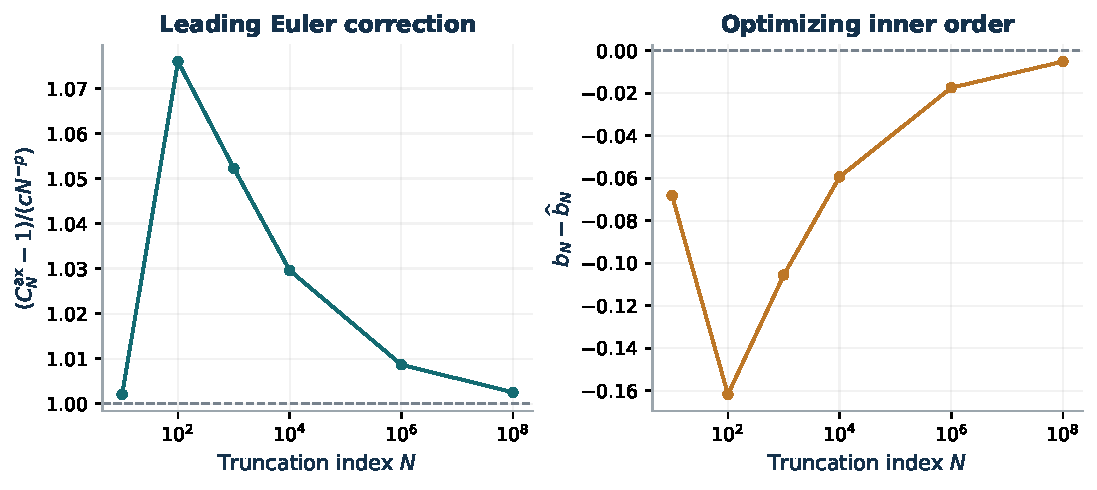
\includegraphics[width=\textwidth]{figures/euler_axis_asymptotics.pdf}
\caption{The optimized axis remainder approaches the proved leading
law, while the inner-order displacement tends to zero. The coefficient
in its finer inverse-logarithmic expansion is large, so moderate
indices need not display the final second-scale amplitude accurately.}
\label{fig:euler-axis}
\end{figure}

The second Euler scale deserves particular care: the proved
coefficient $T(B_0)\approx-2098.43$ makes the approach to its leading
amplitude slow. The data at $N\leq10^8$ are consistent with the first
asymptotic law; they are not a useful basis for fitting the much more
delicate next coefficient. The asymptotic proof identifies that
coefficient through a Mellin integral and uniform domination.

To resolve this slow approach numerically, the additional script
\nolinkurl{code/transition_remainder_diagnostics.py} evaluates the
positive Taylor remainder $\varepsilon_N(\widehat b_N)$ after dividing
by the gamma density at $t=\tfrac12\log N$. It forms no array of
length $N$ and uses stable exponential and hypergeometric remainders.
Define the dimensionless diagnostic
\[
 Q_N=\frac{\varepsilon_N(\widehat b_N)}
              {D_0N^{-\mu}/\sqrt{\log N}}.
\]
The theorem gives $Q_N\to1$ and
$(\log N)(Q_N-1)\to T(B_0)$. The following 75-digit quadratures
show how late these limits become numerically visible.

\begin{table}[htbp]
\centering
\begin{tabular}{rrr}
\toprule
$\log_{10}N$ & $Q_N$ & $(\log N)(Q_N-1)$\\
\midrule
8 & 0.1389757434 & $-15.860653$\\
100 & 0.3477552643 & $-150.184901$\\
1000 & 0.6776397628 & $-742.261877$\\
10000 & 0.9271461038 & $-1677.522954$\\
100000 & 0.9911352486 & $-2041.184436$\\
1000000 & 0.9990912540 & $-2092.464968$\\
\midrule
Proved limit & 1 & $-2098.428735$\\
\bottomrule
\end{tabular}
\caption{Transition-remainder diagnostics at the leading center
$\widehat b_N$. These evaluate the positive remainder at the stated
center. Large exponents are handled through
logarithms and normalized quadrature.}
\label{tab:transition-diagnostics}
\end{table}

At $N=10^8$, an independent direct-axis calculation minus the exact
first Taylor terms agrees with this normalized remainder to relative
error below $10^{-34}$. This is a numerical cross-check of the
implementation, not an interval certificate for the displayed
quadratures. The slow approach reinforces the need for the analytic
proof of the second scale.

\subsection{Pointwise kernel and inverse-series checks}

The kernel calculations solve the two stationary equations in the
scaled coordinates $(c,y)=(Nr,y)$ with 85-digit arithmetic.
At $N=2$ the exact certificate independently proves global optimality.
For other particular finite indices the table records stationary
candidates; the article's global uniqueness theorem is eventual.

\begin{table}[htbp]
\centering
\begin{tabular}{rrrr}
\toprule
$N$ & $Nr$ & $y$ & Stationary kernel value\\
\midrule
2 & 1.7045169541 & 0.2527026784 & 1.1189386860\\
4 & 2.3345294376 & 0.2084961852 & 1.0878146577\\
10 & 3.0411292987 & 0.1758872724 & 1.0689106048\\
100 & 3.8193399906 & 0.1489190557 & 1.0555582496\\
10000 & 3.9397958507 & 0.1453408168 & 1.0538792067\\
\bottomrule
\end{tabular}
\caption{Stationary-kernel diagnostics from the explicit rational
kernel, distinct from the order-averaged constants.}
\label{tab:kernel-diagnostics}
\end{table}

\begin{figure}[htbp]
\centering
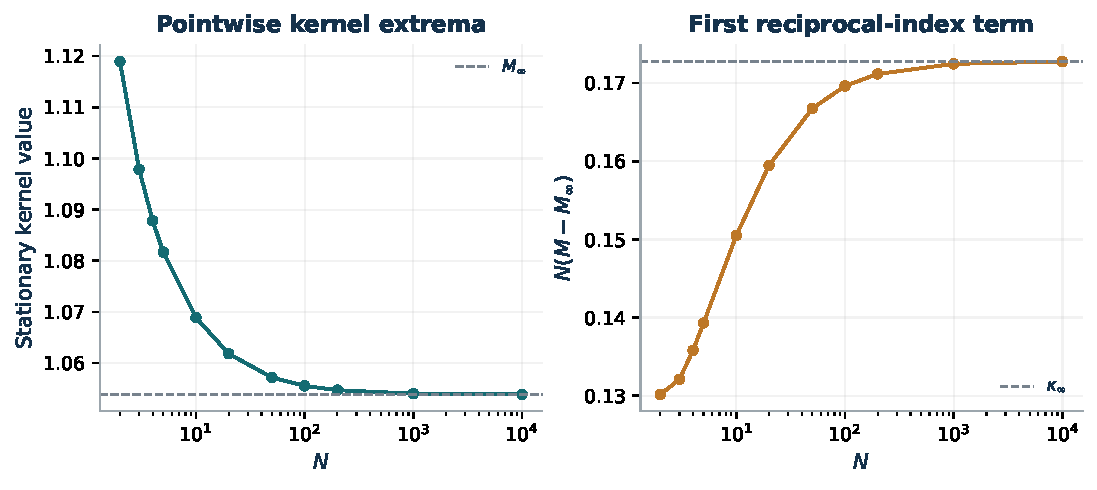
\includegraphics[width=\textwidth]{figures/kernel_limit.pdf}
\caption{Numerical stationary values and their first scaled excess.
The dashed levels are the analytically characterized $M_\infty$ and
$\kappa_\infty$. The proof of convergence covers all global maximizers
and does not depend on this stationary-point computation.}
\label{fig:kernel-limit}
\end{figure}

The inverse-series diagnostics use 360-digit arithmetic for
$A=1.1,2,4,10$ through index 240. Direct Stirling polynomial evaluation
and the independent coefficient recurrence agree to more than 150
relative decimal digits in every tested case. The record also compares
the exact barrier factorization at separate points, the first two
coefficient models, the boundary sums, and the renormalized derivative
sum. An error estimate involving a potentially vanishing cosine is
always displayed in additive normalized form.

\begin{figure}[htbp]
\centering
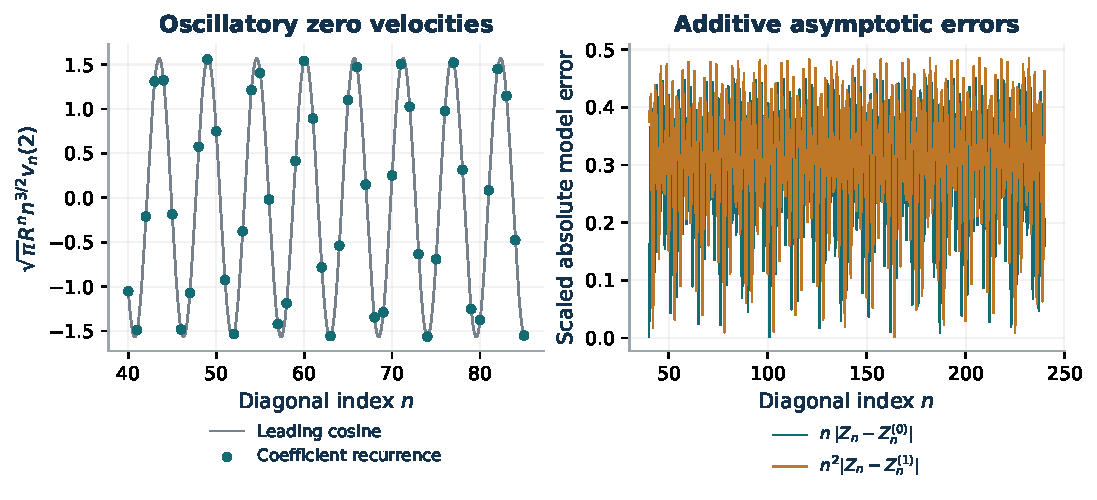
\includegraphics[width=\textwidth]{figures/harmonic_velocity_asymptotics.pdf}
\caption{At $A=2$, coefficients from an independent recurrence follow
the proved oscillatory phase. The right panel plots the errors after
the scalings predicted by the leading and corrected additive
asymptotics. These are finite numerical diagnostics of formulas whose
sheet selection and transfer hypotheses are proved analytically.}
\label{fig:harmonic-velocities}
\end{figure}

\subsection{Lambert roots at the bulk and at both endpoints}

For degrees 12, 30, and 60, the script
\nolinkurl{code/compute_bulk_root_examples.py} isolates every real root
of the exact rational polynomial by symbolic rational interval
arithmetic. Each positive-root interval has width at most $10^{-14}$;
all intervals have multiplicity one. Their midpoints are used only for
plotting. The distribution function is compared with the exact angle
law, and scaled polynomials are compared with the Bessel limit.

\begin{figure}[htbp]
\centering
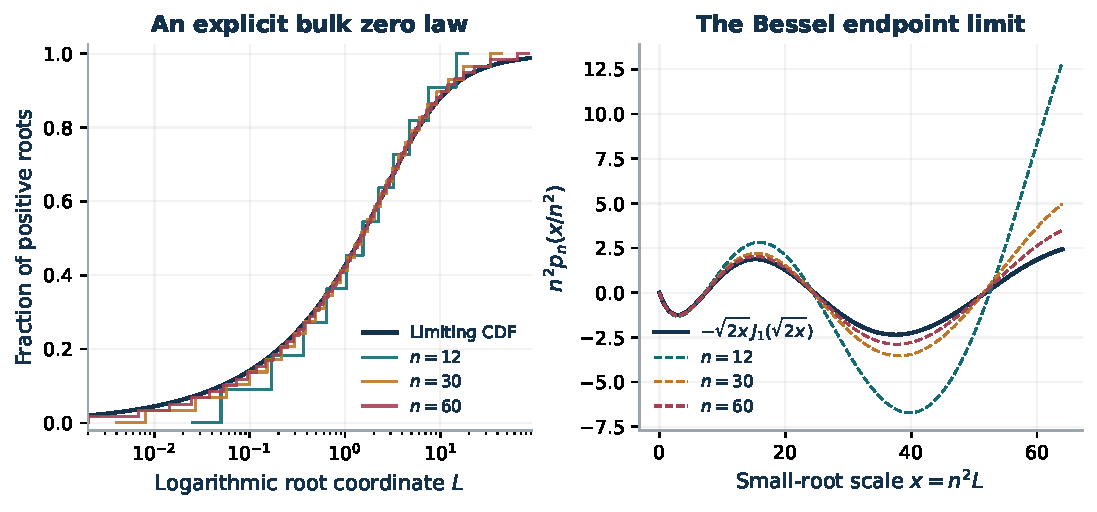
\includegraphics[width=\textwidth]{figures/lambert_bulk_and_bessel.pdf}
\caption{Left: finite positive-root distribution functions, based on
exact rational isolation, approach $\theta(L)/\pi$. Right: the
polynomial scaling at the small-root endpoint approaches the entire
Bessel function in \cref{thm:bessel-edge}. The logarithmic axis on
the left makes both endpoint regions visible.}
\label{fig:bulk-bessel}
\end{figure}

At the opposite endpoint, high-precision evaluation of the reciprocal
polynomial avoids its very large leading powers. The root diagnostics
cover 45 combinations of fixed $j,k$ and $64\leq n\leq1024$.
For $j=k=1$, define
\[
 B_n=n\bigl(X_{n,1,1}-n-\log n-\gamma\bigr),\qquad
 D_n=n^2\bigl(X_{n,1,1}-n-\log n-\gamma-C_0/n\bigr),
\]
where $C_0=-\tfrac32-\zeta(2)-\zeta(3)$.
The next table compares these quantities with their proved limits.

\begin{table}[htbp]
\centering
\begin{tabular}{rrr}
\toprule
$n$ & $B_n$ & $D_n$\\
\midrule
64 & $-4.25307307280$ & 6.01074542118\\
128 & $-4.29945689430$ & 6.08436169117\\
256 & $-4.32307710966$ & 6.12194824995\\
512 & $-4.33499694535$ & 6.14094062226\\
1024 & $-4.34098463490$ & 6.15048715477\\
\midrule
Proved limit & $-4.34699097001$ & 6.16006747240\\
\bottomrule
\end{tabular}
\caption{Largest-root diagnostics. The limit constants come from
exact symbolic formulas and the all-orders theorem.}
\label{tab:cohen-diagnostics}
\end{table}

\begin{figure}[htbp]
\centering
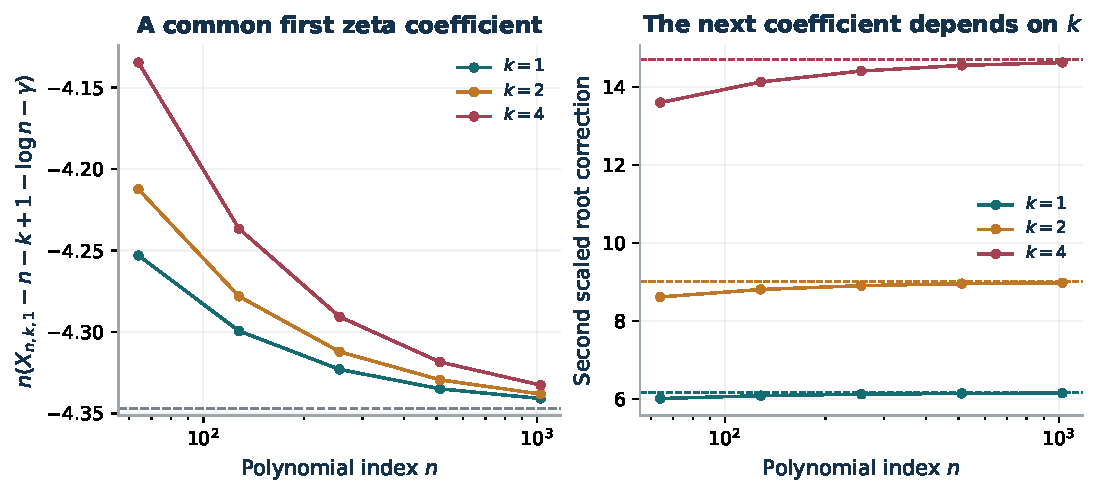
\includegraphics[width=\textwidth]{figures/cohen_extreme_root_coefficients.pdf}
\caption{The first largest-root correction is independent of $k$.
The next one is affine in $k-1$, with the exact expression proved in
\cref{sec:cohen-edges}; its respective limiting levels are dashed.
The numerical root residuals are separate from the analytic root
ordering and remainder proof.}
\label{fig:cohen-coefficients}
\end{figure}

The file \nolinkurl{data/figure_samples.json} also records finite
tests of the newly proposed indexed bulk-phase formula in
\cref{conj:bulk-quantization}. That conjecture is deliberately kept
out of every theorem dependency.

\subsection{Rebuilding and rechecking the package}

The main source is supplied both as \nolinkurl{article.tex} and as
modular sections with \nolinkurl{main.tex}. Run
\nolinkurl{python3 code/assemble_article.py} after editing modules,
then \nolinkurl{latexmk -pdf -halt-on-error article.tex}.
The file \nolinkurl{code/reproduce.py} replays the exact checks by
default; optional flags replay the more expensive diagnostics and
figures. A plain-text readme lists the individual commands and the
versions used. All scripts operate on local files and require no
repository write access or network connection.

The provenance directory pins the source revision and gives Git blob
hashes for retrieved material. A package checksum manifest records the
delivered files. The PDF was compiled from the supplied consolidated
TeX and visually checked after rendering, with particular attention to
long formulas, tables, cross-references, and the distinction between
the proved limits and finite diagnostics.

% ===== sections/09_audit.tex =====
\clearpage
\section{Audit findings and proposed manuscript amendments}
\label{sec:audit}

The source review found several statements whose status can now be
strengthened, two important antecedents that should be cited, and a
small notation error. It did not find a counterexample to the canonical
theorems used as inputs here. In particular, the source material itself
correctly warns that formal critical values do not select an inverse
sheet, that local kernel convergence does not prove convergence of
global maxima, and that floating-point agreement is not an arithmetic
identity proof. Those distinctions should be preserved when the present
results are integrated.

\subsection{Changes in theorem and conjecture status}

\begin{longtable}{@{}>{\raggedright\arraybackslash}p{0.29\textwidth}>{\raggedright\arraybackslash}p{0.65\textwidth}@{}}
\toprule
Source target & Proposed status and supporting result\\
\midrule
\endfirsthead
\toprule
Source target & Proposed status and supporting result\\
\midrule
\endhead
Uniform-bounds report, \texttt{conj:euler-rate}
& Promote the matching global asymptotic to a theorem. Cite
\cref{eul:thm:main,eul:thm:joint-profile,eul:thm:second-term} for
eventual exact axis reduction, the complete near-optimality criterion,
and the sharper next term.\\[5pt]
Sharp-Euler report, \texttt{conj:limit}
& Promote to a theorem with the quantifier covering every sequence of
global maximizers. The proof is \cref{thm:kernel-global-limit};
\cref{thm:kernel-expansion} adds analytic perturbation and eventual
uniqueness and decrease.\\[5pt]
Sharp-Euler report, \texttt{conj:maxima}
& Retain the all-index conjecture. Its uniqueness and interiority
assertion is proved for $N=2$; uniqueness and strict decrease are
proved for all sufficiently large $N$. No verified finite threshold
covers every remaining index.\\[5pt]
The proposed $K_2$ elimination target
& Mark completed. \Cref{thm:M2} proves a unique global interior
maximum and its irreducible degree-seven equation, with an exact
rational certificate.\\[5pt]
Harmonic continuation, \texttt{diag:q:dominance}
& Promote from a conjecture at $A=2$ to the selected-sheet theorem
for every $A>1$, \cref{thm:selected-sheet}. Include the square-root
sign and the radial-slit continuation domain.\\[5pt]
Harmonic continuation, \nolinkurl{diag:q:conditional-asymptotic}
& Remove the conditional hypothesis after the selected-sheet theorem
has been inserted. Credit the existing local calculation and retain
the additive form of the error.\\[5pt]
Diagonal coefficient polynomials
& Identify them explicitly as Cohen's Lambert polynomials up to a
sign. Add the bulk law, largest-root expansion, and Bessel endpoint
limit as further results; do not present the coefficient array itself
as newly discovered.\\
\bottomrule
\end{longtable}

The independent maximum on the axis is unique and nondegenerate at
every integer index, by \cref{eul:prop:axisunique}, and its continuous
interpolation is strictly log-convex. This does not settle all-index
axis reduction for the two-parameter global problem. Similarly, the
analytic dependence of the \emph{kernel} optimum on $1/N$ is a
convergent expansion, whereas the all-orders Lambert-root expansion is
an asymptotic expansion. Their convergence statuses must remain distinct.

\subsection{Two substantive attribution corrections}

\paragraph{The Lambert inverse series.}
In the discussion following the exact generating function, add the
map $\lambda=\log A$, $\sigma=-t/A$, $v=V_A(t)$ to
Kalugin and Jeffrey's equation
$1-e^{-v}+\sigma v-\sigma\lambda=0$
\cite{KaluginJeffrey2012}. Their fixed-$\lambda$ series and radius
criterion are antecedents of the coefficient and radius formulas here.
The repository's missing selected-sheet proof is supplied by the
barrier argument; it should not be described as the first occurrence
of the radius formula.

\paragraph{The Lambert coefficient polynomials.}
Add $L_n(X)=(-1)^np_n(X)$ and the generalized normalization from
Cohen's Proposition 4.8 \cite{Cohen2021}. The real-rooted operator
argument already present in the harmonic report is directly relevant
to Cohen's conjecture. The present interlacing and extreme-root proofs
make the comparison explicit. When quoting the numerical constant in
Cohen's original question \cite{CohenMO2020}, distinguish the two
normalizations:
\begin{align*}
 X_{n,1,1}
 &=n+\log n+\gamma
       -\frac{\frac32+\zeta(2)+\zeta(3)}n+O(n^{-2}),\\
 &=n+H_n
       -\frac{2+\zeta(2)+\zeta(3)}n+O(n^{-2}).
\end{align*}
The difference of $1/2$ in the coefficients comes from
$H_n=\log n+\gamma+1/(2n)+O(n^{-2})$; it is not a discrepancy in
the root asymptotic.

\subsection{A verified notation cleanup}

In the proof of \texttt{rw:thm:transport} in
\nolinkurl{chapters/05-real-positive-kernel.tex}, the instruction to
use the Hurwitz formula ``with $q=n$'' should read ``with $x=n$''.
Here $x$ is the Hurwitz argument; $q$ is the regularizing kernel used
in the neighboring formula. The following sentence refers to boundedness
of $h$, but the regularizer was named $q(t)$, so that occurrence should
read boundedness of $q$. These are notation corrections and do not
change the transport identity or its proof. The package includes a
small unified diff against the pinned source for these two replacements.

\subsection{Integration boundaries and verification status}

The integration notes identify exact source paths and labels, suggest
a placement for the new sections, and list the accompanying verifier
commands. They do not modify the remote repository. The assembled
article is also supplied as modular TeX to make relocation of sections
and theorem environments straightforward.

The exact checks prove finite polynomial identities, finite-field
irreducibility, rational interval enclosures, and the displayed finite
coefficient cancellations. They do not formally verify Rouch\'e's
theorem, the probability representation, singularity transfer, or
asymptotic uniformity. Those claims have the complete mathematical
proofs in the article and the separate review notes in the package.
The source scan and targeted primary-literature comparison support
the stated continuation of this repository; they are not an exhaustive
bibliographic priority search.


% ===== sections/10_research_agenda.tex =====
\section{Further research questions and explicit conjectures}
\label{sec:research-agenda}

The results isolate several precise next problems. The first group
would complete finite-parameter statements already suggested by the
source reports. The later groups ask for uniform transitions or new
structures beyond the results proved here.

\subsection{Complete the finite-index Euler extremum problem}

\begin{conjecture}[Axis reduction at every truncation]
\label{conj:all-index-axis}
For every integer $N\geq1$,
\[
 C_N=\max_{b>0}R_N(0,b),
\]
and the unique maximizer on $a\geq0$, $b>0$ lies on that axis.
\end{conjecture}

The case $N=1$ is part of the known universal-constant theorem;
the present article proves all sufficiently large $N$. The conjecture
is about a global maximum over both orders. It should not be replaced
by a pointwise comparison $R_N(a,b)\leq R_N(0,b)$ at every fixed $b$:
that stronger statement is not the claim and has no such proof here.
A productive approach would combine exact small-index analysis with
an effective, moderately sized threshold in the localization argument.
The relevant difficulties occur outside the eventual competitive band.

An explicit threshold $N_0$ is itself useful. The present split at
$b=2\log N$ produces a slowly vanishing factor
$N^{1-2\log(5/3)}$. Improving this estimate, perhaps with a more
carefully optimized gamma lower-tail bound, would turn the eventual
theorem into a practical enclosure theorem. A finite numerical scan
without a proved tail threshold would not close this question.

\begin{conjecture}[All-index kernel uniqueness and decrease]
\label{conj:all-index-kernel}
For every $N\geq2$, $K_N$ has a unique global maximizer in $(0,1)^2$
and $M_{N+1}<M_N$.
\end{conjecture}

This restates the remaining portion of the sharp-Euler report's
conjecture. The exact $N=2$ elimination and the analytic branch near
$1/N=0$ suggest combining algebraic continuation with certified
boundary exclusions. Monotonicity of the envelope $B_N$ alone does
not prove monotonicity of $M_N$.

\subsection{Refine the gamma-transition asymptotics}

The next Euler scale has the form
$N^{-\mu}(\log N)^{-1/2}$ and carries a large first inverse-logarithmic
coefficient. Determine a uniformly useful approximation across the
moderate-$N$ regime and the true asymptotic regime. The exact positive
remainder integral is a better starting point than subtraction of
nearly equal Euler sums. One target is a resummed transition integral
whose error remains explicit while retaining the slowly decaying tail
responsible for the large coefficient.

For other residual kernels, moment competition may put the analogous
Mellin exponent at an integer. Classify when logarithmic resonances
replace a pure fractional-power correction, and determine the resulting
maximizer displacement. The present proof suggests a general method:
identify the competing exponential moments, localize the parameters,
and analyze the positive remainder near the moving kernel transition.
The exponent and amplitude need to be derived anew for each kernel.

The joint profile in \cref{eul:thm:joint-profile} gives the exact first
loss from leaving the axis. Higher joint terms could quantify stability
of near-optimal order selection at prescribed precision. They should
be stated on explicit joint scales for $a$, $b-\widehat b_N$, and $N$;
pointwise small-$a$ and large-$N$ expansions are not automatically uniform.

\subsection{Determine the arithmetic of the oscillation phase}

For a fixed algebraic value such as $A=2$, is
$\theta(A)/(2\pi)$ irrational? The article proves sign-density
statements in both the rational and irrational cases, so no unproved
phase arithmetic is needed for those theorems. A proof of irrationality
at $A=2$ would give density $1/2$ for each sign and would make rotation
methods available for more precise gap statistics.

Find the least eventual block length that must contain both signs.
The bound $\lfloor\pi/\theta\rfloor+2$ is explicit and gives four at
$A=2$. Whether a smaller block can work is a question about the actual
rotation orbit and its distances from the sign boundaries, together
with the coefficient error. Likewise, quantify the number of indices
where the normalized velocity is unusually small. A relative cosine
approximation is unsuitable for these exceptional indices; the
all-order additive expansion is the available tool.

The finite-part identity for the critically weighted first derivative
can be extended to higher derivative sums. Determine their full
subtraction polynomials in fractional powers of the cutoff, and
identify which finite constants are local Puiseux coefficients.
This should give explicit renormalized Stirling identities, with
ordinary convergence and regularized limits carefully distinguished.

\subsection{A proposed bulk quantization formula}

Let $L_{n,j}$ be the positive zeros of $p_n$ in increasing order,
$\theta_{n,j}=\theta(e^{L_{n,j}})$, and evaluate $u_*,\chi,\chi_1$
at $A=e^{L_{n,j}}$. Put $\phi=-\arg\chi$ as before.
The following indexed refinement is consistent with the finite root
isolations supplied in the package.

\begin{conjecture}[An indexed phase formula in the bulk]
\label{conj:bulk-quantization}
For every fixed $\epsilon\in(0,1/2)$, uniformly for
$\epsilon(n-1)\leq j\leq(1-\epsilon)(n-1)$,
\begin{equation}\label{eq:bulk-quantization-conjecture}
 n\theta_{n,j}+\phi(\theta_{n,j})
 =\pi\left(j+\frac12\right)
   +\frac1n\Im\left(\frac{\chi_1}{\chi}\right)
   +O_\epsilon(n^{-2}).
\end{equation}
\end{conjecture}

The unproved content includes the global root indexing, in particular
the exact shift $j+1/2$. Local transfer locates roots near a half-integer
phase and gives the displayed correction once the index is identified;
the bulk counting theorem alone does not fix that index. One possible
route is to match the Bessel endpoint asymptotic to a uniform interior
expansion in an overlap where $j\to\infty$ and $j/n\to0$.
This is a conjectural asymptotic identity, not a formula used anywhere
in the proofs of this article.

\subsection{Connect the smallest, bulk, and largest root regimes}

The three proved regimes are
\[
 L_{n,j}\asymp n^{-2}\quad(j\text{ fixed from the small end}),
 \qquad L_{n,j}=O(1)\quad(j/n\text{ in the bulk}),
\]
and $X_{n,k,j}\sim n/j$ for $j$ fixed from the large end.
Develop uniform expansions when the root index grows while remaining
$o(n)$. At the large end, the main question is how the expansion around
the $j$th zero of $1/\Gamma(1-w)$ changes when $j$ is no longer fixed.
At the small end, the Bessel zero expansion should be matched to the
singularity-transfer phase. Either transition would sharpen the weak
zero law and give useful discrepancy estimates.

The all-orders largest-root theorem treats fixed positive integer $k$.
Determine uniform ranges of $k=k(n)$, and carefully extend the theorem
to Cohen's derivative interpretation for nonpositive $k$ if desired.
The exact logarithmic change of variables remains a promising starting
point, but the compact-parameter gamma expansion used here does not
justify growing-$k$ or growing-$j$ conclusions.

Recent polynomial-profile methods \cite{JalowyKabluchkoMarynych2026}
may supply another description of the bulk law. Determine whether the
Lambert polynomial family admits a useful limiting Cauchy transform,
free-convolution interpretation, or a potential-theoretic variational
principle. Any such identification should explicitly handle its
degree-dependent differential operator; the fixed-function examples
in the general theory are not automatic substitutes.

\subsection{Return the analytic tools to polylogarithmic identities}

The exact error kernels remain available as certified numerical tools
for cyclotomic and Gaussian polylogarithm identities. The unresolved
mixed $S_6$ reduction is an appropriate arithmetic target, but a
candidate relation requires an independent reduction mechanism such
as iterated-integral relations, a differential identity with controlled
boundary values, or a valid coaction argument. A high-precision integer
relation search alone would still leave a conjecture.

For roots of unity beyond $i$, seek a sector or matrix positivity
statement that replaces the scalar order of the present Gaussian
kernel. At higher depth, identify the correct iterated compensated
differences and prove integrability at each step. The all-depth
oscillation results already in the incoming material concern a
different part of this problem; they should be used with their stated
hypotheses, not treated as a ready-made extension of the present
two-order Euler extremum theorem.

Finally, the exact finite components provide natural formalization
targets: the Euler coefficient identity, the rational derivative and
resultant certificates, finite-field irreducibility, the elementary
real-rooted operators, and the algebra of the first edge coefficients.
A later formal development could then connect them to gamma
integration, Rouch\'e continuation, and singularity transfer. The
package supplies reproducible ordinary proofs and finite arithmetic;
that proposed formal bridge remains future work.

% ===== bibliography.tex =====
\clearpage
\begin{thebibliography}{99}

\bibitem{ProveItSnapshot}
Vladimir Reshetnikov, \emph{Polylogarithms and their Arithmetic Bridges},
ProveIt repository, modular manuscript and editorial material,
revision \texttt{4c173c06cc32c9cea554b39be1837ad2ae897fc1},
October 10, 2026.
\href{https://github.com/VladimirReshetnikov/ProveIt/tree/4c173c06cc32c9cea554b39be1837ad2ae897fc1/Analysis/Polylogarithms/docs/manuscript}{Pinned manuscript directory}.
Especially the real-order Euler and universal-Euler sections, and their
theorem labels \texttt{rw:thm:euler} and
\texttt{univeuler:thm:sharp}.

\bibitem{HarmonicBaseline}
ProveIt harmonic-order geometry continuation,
\emph{Diagonal velocities} and \emph{The diagonal conjecture},
in
\nolinkurl{Analysis/Polylogarithms/docs/reports/lerch-global-phase/continuations/harmonic-order-geometry},
same pinned revision as \cite{ProveItSnapshot}.
\href{https://github.com/VladimirReshetnikov/ProveIt/tree/4c173c06cc32c9cea554b39be1837ad2ae897fc1/Analysis/Polylogarithms/docs/reports/lerch-global-phase/continuations/harmonic-order-geometry}{Pinned continuation directory}.

\bibitem{UniformBoundsIncoming}
\emph{Polylogarithms: Uniform Bounds and Structural Transitions},
incoming ProveIt report, October 10, 2026, archive
\nolinkurl{ProveIt_Polylogarithms_Research_2026-10-10.zip},
directory \nolinkurl{polylogarithms_uniform_bounds_20261010}.
Especially \nolinkurl{sections/euler.tex} and
\nolinkurl{sections/research.tex}, Proposition
\texttt{prop:euler-axis-lower} and Conjecture
\texttt{conj:euler-rate}.
\href{https://github.com/VladimirReshetnikov/ProveIt/tree/4c173c06cc32c9cea554b39be1837ad2ae897fc1/docs/incoming}{Pinned incoming directory}.

\bibitem{SharpEulerIncoming}
\emph{The Sharp Universal Euler Constant for Harmonic Polylogarithms},
incoming ProveIt report, October 10, 2026, archive
\nolinkurl{ProveIt_Sharp_Universal_Euler_2026-10-10.zip}.
Especially \nolinkurl{sections/08-questions.tex} for the limiting-kernel,
uniqueness, monotonicity, and $N=2$ elimination questions.
Same pinned incoming directory as \cite{UniformBoundsIncoming}.

\bibitem{KaluginJeffrey2012}
G.~A. Kalugin and D.~J. Jeffrey,
\emph{Convergence in $\mathbb C$ of series for the Lambert $W$ Function},
arXiv:1208.0754v1, August 2012.
\href{https://arxiv.org/abs/1208.0754}{arXiv record}.
Theorem 1 and equations (1.3), (1.4), (2.2), and (2.9) give the
series and radius criterion used in the attribution comparison.

\bibitem{Cohen2021}
Henri Cohen, \emph{Lambert $W$-Function Branch Identities},
arXiv:2012.11698v2, January 18, 2021.
\href{https://arxiv.org/abs/2012.11698}{arXiv record}.
Proposition 4.8 gives the polynomial identification;
Conjecture 7.1 states the real-root and extreme-root questions.

\bibitem{CohenMO2020}
Henri Cohen,
\emph{Stirling number bounds and polynomials and the Lambert $W$ function},
MathOverflow question 378900, December 14, 2020.
\href{https://mathoverflow.net/questions/378900/stirling-number-bounds-and-polynomials-and-the-lambert-w-function}{Original question}.
The normalization there uses $n+H_n$ in place of $n+\log n+\gamma$.

\bibitem{FlajoletSedgewick2009}
Philippe Flajolet and Robert Sedgewick,
\emph{Analytic Combinatorics}, Cambridge University Press, 2009,
Chapter VI, especially the transfer theorems and multiple-singularity
analysis.
\href{https://algo.inria.fr/flajolet/Publications/AnaCombi/anacombi.html}{Authors' book page and electronic edition}.

\bibitem{Gessel2016}
Ira M. Gessel, \emph{Lagrange Inversion},
Journal of Combinatorial Theory, Series A \textbf{144} (2016), 212--249.
\href{https://arxiv.org/abs/1609.05988}{arXiv:1609.05988}.

\bibitem{DLMFEuler}
NIST Digital Library of Mathematical Functions,
\emph{\S3.9, Acceleration of Convergence}, especially Euler's
transformation.
\url{https://dlmf.nist.gov/3.9}.
Accessed October 10, 2026.

\bibitem{DLMFLambert}
NIST Digital Library of Mathematical Functions,
\emph{\S4.13, Lambert $W$-Function}.
\url{https://dlmf.nist.gov/4.13}.
Accessed October 10, 2026.

\bibitem{DLMFGamma}
NIST Digital Library of Mathematical Functions,
\emph{\S5.11, Asymptotic Expansions}, including the gamma-ratio
expansions in subsection (iii).
\url{https://dlmf.nist.gov/5.11}.
Accessed October 10, 2026.

\bibitem{Weyl1916}
Hermann Weyl, \emph{\"Uber die Gleichverteilung von Zahlen mod. Eins},
Mathematische Annalen \textbf{77} (1916), 313--352.
\href{https://zenodo.org/records/2425535}{Digitized article record}.

\bibitem{Lindemann1882}
Ferdinand Lindemann, \emph{Ueber die Zahl $\pi$},
Mathematische Annalen \textbf{20} (1882), 213--225.
\href{https://eudml.org/doc/157031}{EuDML record}.

\bibitem{DLMFBessel}
NIST Digital Library of Mathematical Functions,
\emph{\S10.2, Definitions}, and \emph{\S10.21, Zeros},
for the Bessel series and the positive zeros of $J_k$.
\url{https://dlmf.nist.gov/10.2};
\url{https://dlmf.nist.gov/10.21}.
Accessed October 10, 2026.

\bibitem{JalowyKabluchkoMarynych2026}
Jonas Jalowy, Zakhar Kabluchko, and Alexander Marynych,
\emph{Zeros and Exponential Profiles of Polynomials II: Examples},
Constructive Approximation (2026),
\href{https://doi.org/10.1007/s00365-026-09775-2}{doi:10.1007/s00365-026-09775-2}.
Relevant general context for polynomial zero limits; the ordinary
Stirling and Touchard families discussed there should not be identified
with Cohen's Lambert polynomials without a separate argument.

\end{thebibliography}
\end{document}
